%% Copyright 2012-2014 by abnTeX2 group at http://abntex2.googlecode.com/ 
% ------------------------------------------------------------------------
% ------------------------------------------------------------------------
% abnTeX2: Modelo de Trabalho Acadêmico (tese de doutorado, dissertacao de
% mestrado e trabalhos monográficos em geral) em conformidade com 
% ABNT NBR 14724:2011: Informação e documentação - Trabalhos acadêmicos -
% Apresentação
% ------------------------------------------------------------------------
% ------------------------------------------------------------------------

\documentclass[
	% -- opções da classe memoir --
	12pt,				% tamanho da fonte
	openright,			% capítulos começam em pág ímpar (insere página vazia caso preciso)
	oneside,			% para impressão em verso e anverso. Oposto a oneside
	a4paper,			% tamanho do papel. 
	% -- opções da classe abntex2 --
	%chapter=TITLE,		% títulos de capítulos convertidos em letras maiúsculas
	%section=TITLE,		% títulos de seções convertidos em letras maiúsculas
	%subsection=TITLE,	% títulos de subseções convertidos em letras maiúsculas
	%subsubsection=TITLE,% títulos de subsubseções convertidos em letras maiúsculas
	% -- opções do pacote babel --
	english,			% idioma adicional para hifenização
	brazil				% o último idioma é o principal do documento
	]{abntex2}

% ---
% Pacotes
% ---
\usepackage{lmodern}			% Usa a fonte Latin Modern			
\usepackage[T1]{fontenc}		% Seleção de códigos de fonte.
\usepackage[utf8]{inputenc}		% Codificação do documento (conversão automática dos acentos)
\usepackage{lastpage}			% Usado pela Ficha catalográfica
\usepackage{indentfirst}		% In denta o primeiro parágrafo de cada seção.
\usepackage{color}				% Controle das cores
\usepackage{graphicx}			% Inclusão de gráficos
\usepackage{microtype} 			% para melhorias de justificação
\usepackage{comment}           %para inserir blocos de comentário
\usepackage{mathptmx}
\usepackage{amsmath}
\usepackage{mathtools}
\usepackage{empheq}
\usepackage[brazilian,hyperpageref]{backref}	 % Paginas com as citações na bibl
\usepackage[alf]{abntex2cite}	% Citações padrão ABNT
\usepackage{etoolbox}


% --- 
% CONFIGURAÇÕES DE PACOTES
% --- 

\graphicspath{ {img/} } % Local das imagens
\apptocmd{\sloppy}{\hbadness 10000\relax}{}{} %



% ---
% Macros e funções
% ---

% Utilizado para por bordas nos protocolos
\newcommand*\widefbox[1]{\fbox{\hspace{2em}#1\hspace{2em}}}

\newcommand{\bordaProtocolo}[1]{
    \centering
    \framebox{\parbox{\dimexpr\linewidth-15\fboxsep-2\fboxrule}{\itshape%
        \vspace{2mm}
        #1
        \vspace{2mm}
    }}
}


% Configurações do pacote backref
% Usado sem a opção hyperpageref de backref
\renewcommand{\backrefpagesname}{Citado na(s) página(s):~}
% Texto padrão antes do número das páginas
\renewcommand{\backref}{}
% Define os textos da citação
\renewcommand*{\backrefalt}[4]{
	\ifcase #1 %
		Nenhuma citação no texto.%
	\or
		Citado na página #2.%
	\else
		Citado #1 vezes nas páginas #2.%
	\fi}%
% ---


%%%%%%%%%%%%%%%%%%%%%%%%%%%%%%%%%%%%%%%%%%%%%%%%%%%%%%%%%%%%%%%%%%%%%%%%%%%%%%%%%%%%%%%%%%%%%
%                                                                                           %
%                           Construindo elementos pré textuais                              %
%                                                                                           %
%%%%%%%%%%%%%%%%%%%%%%%%%%%%%%%%%%%%%%%%%%%%%%%%%%%%%%%%%%%%%%%%%%%%%%%%%%%%%%%%%%%%%%%%%%%%%

% ---
% Informações de dados para CAPA e FOLHA DE ROSTO
% ---

\titulo{Implementação e Adaptação de um Sistema de Arquivos Distribuídos Móvel Adaptável e Flexível para Dispositivos Móveis}
\autor{Gabriel Henrique Martinez Saraiva}
\local{São José do Rio Preto}
\data{2014}
\orientador[Prof. Dr.]{Renata Spolon Lobato}

%%inserir caso ouver%% -> \coorientador{}


\instituicao{%
  Universidade Estadual Paulista "Júlio de Mesquita Filho" (UNESP)
  \par
  Instituto de Biociências, Letras e Ciências Exatas (IBILCE)
  \par
  Bacharelado em Ciência da Computação}
  
\tipotrabalho{Monografia de Qualificação}
% O preambulo deve conter o tipo do trabalho, o objetivo, 
% o nome da instituição e a área de concentração 
\preambulo{Monografia ao Departamento de Ciências de  Computação  e  Estatística  do  Instituto  de Biociências,  Letras  e  Ciências  Exatas  da Universidade  Estadual  Paulista  ”Júlio  de  Mesquita Filho”,  como  parte  dos  requisitos  necessários  para obtenção do título de "Bacharel" pelo curso de Bacharel em Ciência  da Computação da UNESP}
% ---

% informações do PDF
\makeatletter
\hypersetup{
     	%pagebackref=true,
		pdftitle={\@title}, 
		pdfauthor={\@author},
    	pdfsubject={\imprimirpreambulo},
	    pdfcreator={LaTeX with abnTeX2},
		pdfkeywords={abnt}{latex}{abntex}{abntex2}{trabalho acadêmico}, 
		colorlinks=true,       		% false: boxed links; true: colored links
    	linkcolor=blue,          	% color of internal links
    	citecolor=blue,        		% color of links to bibliography
    	filecolor=magenta,      		% color of file links
		urlcolor=blue,
		bookmarksdepth=4
}
\makeatother
% --- 


% ---
% Configurações de aparência do PDF final

% alterando o aspecto da cor azul
\definecolor{blue}{RGB}{41,40,40}

% --- 
% Espaçamentos entre linhas e parágrafos 
% --- 

% O tamanho do parágrafo é dado por:
\setlength{\parindent}{1.3cm}

% Controle do espaçamento entre um parágrafo e outro:
\setlength{\parskip}{0.2cm}  % tente também \onelineskip

% ---
% compila o indice
% ---
\makeindex
% ---


% ----
% Início do documento
% ----
\begin{document}

% Retira espaço extra obsoleto entre as frases.
\frenchspacing 

% ----------------------------------------------------------
% ELEMENTOS PRÉ-TEXTUAIS
% ----------------------------------------------------------
% \pretextual

% ---
% Capa
% ---
\imprimircapa
% ---

% ---
% Folha de rosto
% (o * indica que haverá a ficha bibliográfica)
% ---
\imprimirfolhaderosto
% ---

% ---
% Inserir a ficha bibliográfica
% ---

% Isto é um exemplo de Ficha Catalográfica, ou ``Dados internacionais de
% catalogação-na-publicação''. Você pode utilizar este modelo como referência. 
% Porém, provavelmente a biblioteca da sua universidade lhe fornecerá um PDF
% com a ficha catalográfica definitiva após a defesa do trabalho. Quando estiver
% com o documento, salve-o como PDF no diretório do seu projeto e substitua todo
% o conteúdo de implementação deste arquivo pelo comando abaixo:
%
% \begin{fichacatalografica}
%     \includepdf{fig_ficha_catalografica.pdf}
% \end{fichacatalografica}

%%%%%%%%%%%%%% Qualificação não é catalogada %%%%%%%%%%%%%%%%%%%%%%%%%%%%%%%%%%%%%%%%


%
%\begin{comment}
%
%\begin{fichacatalografica}
	%\vspace*{\fill}					% Posição vertical
	%\hrule							% Linha horizontal
	%\begin{center}					% Minipage Centralizado
	%\begin{minipage}[c]{12.5cm}		% Largura
%	
	%\imprimirautor
%	
	%\hspace{0.5cm} \imprimirtitulo  / \imprimirautor. --
%	\imprimirlocal, \imprimirdata-
%	
%	\hspace{0.5cm} \pageref{LastPage} p. : il. (algumas color.) ; 30 cm.\\
%	
%	\hspace{0.5cm} \imprimirorientadorRotulo~\imprimirorientador\\
%	
%	\hspace{0.5cm}
%	\parbox[t]{\textwidth}{\imprimirtipotrabalho~--~\imprimirinstituicao,
%	\imprimirdata.}\\
%	
%	\hspace{0.5cm}
%		1. Palavra-chave1.
%		2. Palavra-chave2.
%		I. Orientador.
%		II. Universidade xxx.
%		III. Faculdade de xxx.
%		IV. Título\\ 			
%	
%	\hspace{8.75cm} CDU 02:141:005.7\\
%	
%	\end{minipage}
%	\end{center}
%	\hrule
%\end{fichacatalografica}

%\end{comment}
% ---

% ---
% Inserir errata
% ---

%%%%%%%%%%%%%%%%%%%%%%%%%%%%%%%%%%% sem errata por enquanto %%%%%%%%%%%%%%%%%%%%%%%%%%%%%%%
\begin{comment}

\begin{errata}

\end{errata}

\end{comment}
% ---

% ---
% Inserir folha de aprovação
% ---

% Isto é um exemplo de Folha de aprovação, elemento obrigatório da NBR
% 14724/2011 (seção 4.2.1.3). Você pode utilizar este modelo até a aprovação
% do trabalho. Após isso, substitua todo o conteúdo deste arquivo por uma
% imagem da página assinada pela banca com o comando abaixo:
%
% \includepdf{folhadeaprovacao_final.pdf}
%

%%%%%%%%%%%%%%%%%%%%%%%% sem aprovação por enquanto %%%%%%%%%%%%%%%%%%%%%%%%%%%%%%%%%%%%%
\begin{comment}

\begin{folhadeaprovacao}

  \begin{center}
    {\ABNTEXchapterfont\large\imprimirautor}

    \vspace*{\fill}\vspace*{\fill}
    \begin{center}
      \ABNTEXchapterfont\bfseries\Large\imprimirtitulo
    \end{center}
    \vspace*{\fill}
    
    \hspace{.45\textwidth}
    \begin{minipage}{.5\textwidth}
        \imprimirpreambulo
    \end{minipage}%
    \vspace*{\fill}
   \end{center}
        
   Trabalho aprovado. \imprimirlocal, 24 de novembro de 2012:

   \assinatura{\textbf{\imprimirorientador} \\ Orientador} 
   \assinatura{\textbf{Professor} \\ Dr. Aleardo Manacero Jr.}
   \assinatura{\textbf{Professora} \\ Dra. Adriana Adriana Barbosa Santos}
  
      
   \begin{center}
    \vspace*{0.5cm}
    {\large\imprimirlocal}
    \par
    {\large\imprimirdata}
    \vspace*{1cm}
  \end{center}
  
\end{folhadeaprovacao}
% ---
\end{comment}

% ---
% Dedicatória
% ---
\begin{dedicatoria}
   \vspace*{\fill}
   \centering
   \noindent
   \textit{ Dedico esse trabalho a todos que algum dia, de alguma forma colaboraram para que se tornasse realidade.} \vspace*{\fill}
\end{dedicatoria}
% ---

% ---
% Agradecimentos
% ---
%%%%%%%%%%%%%%%%%%%%%% agradecimentos %%%%%%%%%%%%%%%%%%%%%%%%%%%%%%%%%
\begin{comment}

\begin{agradecimentos}

Agradeço a todos que algum dia, de alguma forma colaboraram para que se tornasse realidade.

\end{agradecimentos}

\end{comment}

% ---

% ---
% Epígrafe
% ---
\begin{epigrafe}
    \vspace*{\fill}
	\begin{flushright}
		\textit{"E quantas vezes você disse que não aguentava mais,\\ mas continuou seguindo em frente?"} \\
		-autor desconhecido
	\end{flushright}
\end{epigrafe}
% ---

% ---
% RESUMOS
% ---

% resumo em português
\setlength{\absparsep}{18pt} % ajusta o espaçamento dos parágrafos do resumo
\begin{resumo}
 
    Esse trabalho faz um levantamento bibliográfico sobre sistemas distribuídos, sistemas de arquivos distribuídos, Android e dispositivos móveis e sobre o uso de chamada de procedimentos remotos. 
 
    Servindo como fundamentação teoria, o levantamento bibliográfico embasa a execução do trabalho, que é focado basicamente em duas grandes sessões, sendo a primeira parte do trabalho sobre a padronização do FlexA (\textit{Flexible and Adaptable Distributed File System}), desenvolvido no Grupo de Sistemas Paralelos e Distribuídos (GSPD), desenvolvendo uma documentação coesa baseada em diagramas de classes, casos de uso funcionais, e protocolos de comunicação. Essa documentação tem como função permitir o progresso futuro do projeto. E na segunda parte estão a adaptação do módulo servidor para que esse seja compatível as interfaces de comunicação e protocolos propostos além da implementação de um cliente Android para que o sistema possa ser utilizado de maneira mais fácil e dinâmica pelos usuários.

 \textbf{Palavras-chaves}: Android, chamada de procedimentos remotos, sistemas distribuídos, sistemas de arquivos distribuídos.
\end{resumo}

% resumo em inglês
\begin{resumo}[Abstract]
 \begin{otherlanguage*}{english}
 
    TODO - PEGAR COM O VICTOR HUGO CANDIDO!!!!\\
    TODO - PEGAR COM O VICTOR HUGO CANDIDO!!!!\\
    TODO - PEGAR COM O VICTOR HUGO CANDIDO!!!!\\
    TODO - PEGAR COM O VICTOR HUGO CANDIDO!!!!\\
    TODO - PEGAR COM O VICTOR HUGO CANDIDO!!!!\\
    TODO - PEGAR COM O VICTOR HUGO CANDIDO!!!!\\
    TODO - PEGAR COM O VICTOR HUGO CANDIDO!!!!
    

   \vspace{\onelineskip}
 
   \noindent 
   \textbf{Key-words}: mobile devices, distributed file systems
 \end{otherlanguage*}
\end{resumo}


% ---
% inserir lista de ilustrações
% ---
\pdfbookmark[0]{\listfigurename}{lof}
\listoffigures*
\cleardoublepage
% ---
% inserir lista de tabelas
% ---
\pdfbookmark[0]{\listtablename}{lot}
\listoftables*
\cleardoublepage
% ---

% ---
% inserir lista de abreviaturas e siglas
% ---
\begin{siglas}
\item SD - Sistema Distribuído
\item MD5 - \textit{Message-Digest algorithm 5}
\item SHA - \textit{Secure Hash Algorithm}
\item SA - Sistemas de Arquivos
\item EXT2 - \textit{second extended filesystem}
\item EXT3 - \textit{third extended filesystem}
\item EXT4 - \textit{fourth extended filesystem}
\item FAT - \textit{File Alocation Table}
\item NTFS - \textit{New Technology File System}
\item SAD - Sistemas de Arquivos Distribuídos
\item NFS - \textit{Network File System} 
\item ACL - \textit{Access Control List}


\end{siglas}
% ---

\begin{comment}
% ---
% inserir lista de símbolos
% ---
\begin{simbolos}


\end{simbolos}
% ---
\end{comment}


% ---
% inserir o sumario
% ---
\pdfbookmark[0]{\contentsname}{toc}
\tableofcontents*
\cleardoublepage
% ---



% ----------------------------------------------------------
% ELEMENTOS TEXTUAIS
% ----------------------------------------------------------
\textual
% Revisado por Gabriel Saraiva - 14:02

\chapter{Introdução}
\label{cap1}

    A rápida evolução da computação, devido a concorrência entre os fabricantes e sua demanda perene, possibilitou o barateamento e o aumento na capacidade dos sistemas computacionais. Resultado de grandes avanços tecnológicos, dos microprocessadores aliado aos sistemas de conexão e redes, a computação se tornou onipresente em muitos campos de nossa sociedade, como destacado por ~\cite{tanenbaum}.

    A evolução desses sistemas proporcionou a solução de problemas maiores e mais complexos, que comumente não são possíveis de serem solucionados com dispositivos isolados. Para a solução desses problemas são utilizados sistemas distribuídos, onde sistemas computacionais diversos cooperam, se comunicando via redes de computadores e internet para atingir um objetivo comum ~\cite{coulouris}.

    Dentro da computação distribuída, como é necessário armazenar esses dados e fazer o compartilhamento deles, existem os sistemas de arquivos distribuídos, que são responsáveis por fornecer acesso aos dados de forma constante e confiável. Nesse trabalho será tratado o FlexA (\textit{Flexible and Adaptable Distributed File System}), desenvolvido no GSPD (Grupo de Sistemas Paralelos e Distribuídos) da UNESP.


\section{Motivação}

    Dentre os fatores que motivam esse trabalho estão a necessidade de tornar o FlexA um sistema mais fácil de ser expandido no futuro, através de  interfaces que tornem o projeto mais aberto e flexível com relação ao desenvolvimento e arquitetura. Também, aproveitando a grande popularização de dispositivos de computação móvel como, por exemplo, \textit{tablets} e \textit{smartphones}, que com a presença e uso constante desses dispositivos o FlexA poderia ser utilizado pelo usuário de forma prática e rápida.

\section{Objetivos}

    Os objetivos gerais desse trabalho são adaptar as interfaces de comunicação do FlexA, de modo a remodelar interfaces de comunicação entre cliente e servidor, e implementar uma versão do módulo cliente do sistema para dispositivos móveis que utilizem Android.

    Os objetivos específicos são a implementação das operações desconectadas que são responsáveis por gerenciar o FlexA enquanto estiver desconectado e sincronizá-lo ao conectar novamente com os servidores; implementação de um módulo de controle de falhas de conexão, e mecanismos mínimos de segurança dos dados e da comunicação com os servidores, utilização de criptografia e chaves de identificação. Como esses dispositivos possuem uma capacidade de armazenamento menor, existe a necessidade de um melhor gerenciamento dos arquivos residentes na memória cache do sistema de arquivo distribuído (SAD).

\section{Organização do texto}

    No trabalho estão, além dessa introdução, no capítulo \ref{cap2} a fundamentação teórica sobre a qual o trabalho foi desenvolvido, com o estudo de sistemas distribuídos, sistemas de arquivos distribuídos, chamada de procedimentos remotos e também sobre Android e dispositivos móveis. No capítulo \ref{cap3} é descrito o desenvolvimento do projeto e são mostrados os diversos mecanismos utilizados e implementados. O capítulo \ref{cap4} apresenta os cenários de testes utilizados, e os testes realizados para validação do projeto. Por fim, no capítulo \ref{cap5} são feitos comentários sobre a execução do projeto desenvolvido e dos testes realizados, e são apresentadas as dificuldades e novos caminhos para projetos futuros.
    
%% Revisado por Gabriel Saraiva
%% Revisado por Renata

\chapter{Revisão Bibliográfica}
\label{cap2}

Neste capítulo são apresentados os conceitos sobre Sistemas de Arquivos Distribuídos (com foco na comunicação entre cliente e servidor), e principalmente dispositivos móveis, apresentando suas restrições.


\section{Sistemas Distribuídos}

    Segundo ~\cite{tanenbaum}, um Sistema Distribuído (SD) é um conjunto de computadores independentes que se apresenta aos usuários como um sistema único e coerente, ocultado detalhes da implementação que não são úteis aos usuários. Ainda sim um sistema distribuído pode ser definido de acordo com ~\cite{coulouris} como um sistema onde os componentes computacionais, tanto os de \textit{hardware} como os de \textit{software}, se comunicam e coordenam suas ações através de mensagens transmitidas por uma ou mais redes de computadores, independente da distância entre seus componentes. Essas características, agregam diversos desafios na implementação de sistemas distribuídos. De acordo com ~\cite{coulouris} esses desafios são:
    
    \subsection{Heterogeneidade}
        Como esses sistemas muitas vezes são compostos por \textit{hardwares} e arquiteturas diferentes, diversos sistemas operacionais e \textit{softwares} desenvolvido por diferentes equipes e muitas vezes com configurações distintas entre outros fatores. Dessa forma é de grande importância que todo o sistema seja baseado em protocolos compatíveis que possam gerenciar essas diferenças e fornecer ao usuário um ambiente único e coeso.
    
    \subsection{Abertura}
        Um sistema é dito aberto quando suas interfaces de comunicação ou de desenvolvimento são acessíveis e programas podem ser feitos ou alterados por terceiros para que sejam compatíveis com esse sistema. Os grandes desafios para criar sistemas abertos são: fornecer principais interfaces publicamente, mecanismos de comunicação uniforme para acesso a recursos compartilhados e por fim, realizar os testes necessários para que esse sistema se comporte como esperado e seja compatível com o padrão publicado.
    
    \subsection{Segurança}
Um dos grandes desafios de sistemas distribuídos é manter a segurança do próprio sistema de modo a manter a disponibilidade do serviço a seus clientes, confidencialidade dos dados que ele armazena ou processa e não menos importante a integridade do sistema e dos dados que estão no SD. Esse tópico é de grande importância na maioria dos SD disponíveis pois afeta principalmente a disponibilidade do serviço aos usuários e a confiança que o usuário tem sobre o serviço ~\cite{coulouris}.
    
    \subsection{Escalabilidade}
        Um sistema é dito escalável se seu desempenho cresce proporcionalmente aos recursos que são inserido no SD, sem perda de qualidade ou desempenho do serviço. Essa característica é muito importante para que o sistema continue operando em cenários que exijam mais recursos do que o cenário inicial para o qual o sistema implantado. Embora pareça um desafio fácil de solucionar, como mostrado em ~\cite{coulouris}, as soluções desses desafios não são sempre triviais, como por exemplo gerenciar a perda de desempenho do sistema ao aumentar o número de servidores e clientes em uma rede, ou manter a latência dentro de um patamar aceitável com o crescimento do número de servidores e a distância entre eles.
    
    \subsection{Tratamento de falhas}

        Como o sistema é distribuído, falhas tendem a não comprometer a totalidade do sistema, afetando apenas alguns pontos  por vez enquanto outros continuam operando. Mas isso torna essas falhas complexas de serem tratadas, para que o sistema volte a operar como esperado ~\cite{coulouris}. Para tratar essas falhas são utilizadas as seguintes técnicas:
        \begin{enumerate}
    
            \item Detecção de falha: Erros de transmissão por exemplo podem ser detectados e facilmente corrigidos através de mecanismos próprios e algoritmos bem conhecidos como por exemplo o os algoritmos de \textit{hash} \textit{Message-Digest algorithm 5} (MD5) e o \textit{Secure Hash Algorithm} (SHA);
            
            \item Mascaramento de falha: Essa técnica consiste não em solucionar o problema mas aumentar a resistência do sistema as falhas, como por exemplo replicar informações servidores e retransmitir mensagens danificadas;
            
            \item Tolerância a falhas: Nem sempre é possível construir sistemas a prova de falhas, sendo muito mais simples e barato projetá-los para tolerar algumas falhas até certo ponto e depois disso informar o usuário sobre a falha ocorrida. Um exemplo clássico citado em ~\cite{coulouris} é o do navegador \textit{web} que, após um certo número de tentativas sem sucesso de carregar uma página \textit{web}, desiste de tentar carregar a página e informa o erro ao usuário;
            
            \item Redundância: Outra forma de tornar o sistema mais tolerante a falhas é acrescentar redundância ao sistema, para que caso uma parte falhe, outras partes detectem essa falha e assumam as tarefas do módulo que falhou sem prejudicar o funcionamento do sistema como um todo. Exemplos são servidores replicados e múltiplas rotas para um destino ~\cite{coulouris};
            
            \item Recuperação de falhas: Mesmo que não seja possível evitar falhas, é importante que o sistema seja capaz de se recuperar delas. Um exemplo disso é o uso de \textit{logs} nos sistemas de arquivos locais e de servidores que fazem sincronismo com seus pares após alguma falha que cause a falta de sincronismo do sistema ~\cite{coulouris};
            
        \end{enumerate}
    
    
    \subsection{Transparência}
    
        Dentre diversos recursos para fornecer um sistema coerente ao usuário e esconder dele a complexidade do sistema, estão os conceitos de transparência. Como apresentado em ~\cite{tanenbaum}, é possível listar os conceitos de transparência que o projeto atual utiliza de forma mais intensiva, como por exemplo:
    
        \begin{itemize}
            \item Transparência de acesso: toda a complexidade no acesso dos dados é escondida do usuário;
            
            \item Transparência de localização: oculta do usuário a localização dos recursos distribuídos;
            
            \item Transparência de migração: é responsável por omitir do usuário detalhes referente a migração dos dados para outras localidades físicas e lógicas;
            
            \item Transparência de replicação: ocultam do usuário os mecanismos de replicação dos dados;
            
            \item Transparência de falhas: esconde do usuário e tenta solucionar os problemas referentes as falhas que ocorrem no sistema, de modo a evitar com que o usuário seja prejudicado quando uma falha acontece no sistema, como visto anteriormente, detectando, mascarando, tolerando, usando módulos redundantes ou até mesmo recuperando o sistema quando possível.
        \end{itemize}
    
        Embora todas essas camadas de transparência sejam desejadas nem sempre é possível fornecer transparência total ao usuário por questões práticas, como usabilidade, complexidade na implementação e a degradação do desempenho que elas geram.

\section {Sistema de Arquivos}
    Sistemas de arquivos (SA) foram criados para oferecer ao programador uma interface padronizada de acesso aos arquivos, independente de como e onde estão armazenados ~\cite{coulouris} dentro dos dispositivos locais. 
    Além dos dados (arquivos propriamente ditos), sistemas de arquivos devem armazenar também os metadados, que são informações sobre os dados (arquivos). Esses metadados comumente são os seguintes ~\cite{coulouris} (adaptado):
    
    \begin{itemize}
        \item Nome do arquivo;
        \item Dono do arquivo;
        \item Grupo do arquivo;
        \item Horário de criação;
        \item Horário de acesso;
        \item Horário de modificação;
        \item Horário de alteração de atributo;
        \item Contagem de referências;
        \item Tipo do arquivo (diretório, arquivo, \textit{link});
        \item Lista de permissões de acesso.
    \end{itemize}
    
    Além de gerenciar como os arquivos são armazenados e acessados, cabe ao sistema de arquivos a responsabilidade de fazer o controle de acesso dos arquivos que ele armazena, restringindo o acesso conforme as regras definidas pelos usuários ou sistema. Essas regras normalmente podem ser expressas pelos acessos de leitura, escrita e execução dos arquivos.
    
    Em um sistema de arquivos convencional todo acesso aos arquivos é controlado pelo \textit{kernel} do sistema operacional. O tratamento do acesso é feito pelo próprio núcleo do sistema. Em sistemas distribuídos esse tratamento é feito de forma diferente. Isso será abordado na sessão de Sistemas de Arquivos Distribuídos na sessão \ref{sad}.
    
    Exemplos de sistemas de arquivos são: os \textit{extended file systems} (EXT2, EXT3, EXT4), XFS, ReiserFS, \textit{Journaling FileSystem} (JFS) para sistemas \textit{Unix-like} e não menos importantes os \textit{File Allocation Table} (FAT16, FAT32, FAT32EX), e o \textit{New Technology File System} (NTFS) para sistemas da Microsoft.


	\section{Sistemas de Arquivos Distribuídos} \label{sad}

	 Sistemas de Arquivos Distribuídos (SAD) são sistemas que oferecem compartilhamento desses arquivos através de redes, fornecendo desempenho, integridade, confidencialidade e disponibilidade equivalentes ou superiores aos sistemas de arquivos tradicionais ~\cite{coulouris}, permitindo que programas armazenem e acesses os arquivos remotos como se fossem locais, fornecendo aos usuários liberdade para acessar seus arquivos independente do computador que utilizem, desde que dentro de uma rede local ou que tenha acesso ao sistema de arquivos distribuído utilizado.
	 
	 Um SAD básico pode ser descrito como é encontrado em ~\cite{coulouris}, em que o objetivo é simplesmente simular o funcionamento de um sistema de arquivos tradicional para que programas clientes executem em computadores remotos. Esses não fazem o uso de sistema de réplicas, nem suportam sistemas multimídia que exigem grandes fluxos de dados e a capacidade de fazer a entrega desses dados com uma temporização bem limitada.
	 Analisado por essa perspectiva que é apresentada em ~\cite{coulouris}, o sistema de arquivos distribuído que é alvo desse trabalho pode ser considerado um SAD não básico, pois implementa vários recursos não encontrados em sistemas básicos. Esse sistema será apresentado na seção \ref{flexa}.
	 
	Assim, para projetar um sistema de arquivos distribuído de alto desempenho capaz de armazenar grandes quantidades de dados e que suporte escrita e leitura em larga escala, é necessário resolver diversos problemas, como balanceamento de carga, confiabilidade, disponibilidade, segurança, e concorrência de acesso aos dados ~\cite{coulouris}.
	 
	 
	 A seguir são elencados alguns sistemas de arquivos distribuídos que são referências clássicas e foram a base do desenvolvimento desse trabalho.
	


	 
	\subsection{\textit{Network File System} (NFS)}
	
O \textit{Network File System} (NFS) foi projetado pela \textit{Sun Microsystems} para funcionar em suas estações de trabalho. Atualmente é compatível com quase todos os sistemas operacionais de grande uso. Foi lançado como o primeiro SAD destinado a ser um produto final e ter suas interfaces e protocolo abertos ao público. Sua grande compatibilidade somada a premissa de fornecer acesso transparente aos arquivos remotos através do uso das chamadas ao \textit{Virtual File System} (VSF) e do uso de \textit{Remote Procedure Call} RPC foram os grandes fatores que contribuíram para seu sucesso e sua popularização ~\cite{coulouris}. Sua arquitetura é apresentada na Figura \ref{fig:arquiteturaNFS} .
	
    	\begin{figure}[!ht]
            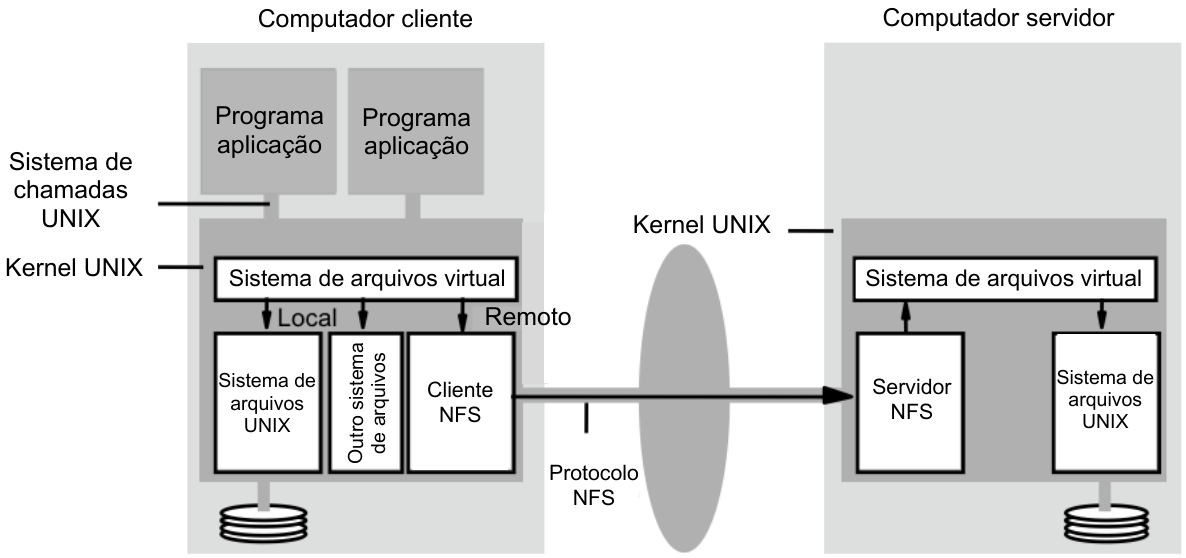
\includegraphics[width=12cm]{arquiteturaNFS.png}
            \caption{Arquitetura do NFS ~\cite{coulouris}}
            \label{fig:arquiteturaNFS}
        \end{figure}
    
    Seu projeto independente do estado do sistema (\textit{stateless}) basicamente inviabiliza a utilização de mecanismos para recuperação de falhas ~\cite{coulouris}.
    
    O uso de memória \textit{cache} no servidor tenta antecipar o que o cliente irá solicitar e já manter esses dados na memória para que, quando o cliente solicitá-los, possam ser entregues sem o gargalo de acesso ao disco. O uso de \textit{cache} na escrita se baseia em manter o arquivo na memória por um tempo sem que o cliente o altere e só então gravar o arquivo no disco. Ainda sim existe a operação \textit{sync} que grava as informações pendentes no disco a cada 30 segundos.
    Quanto a \textit{cache} no cliente é feita através da datas de modificação dos arquivos. Caso haja discrepâncias entre cliente e servidor, o cliente é atualizado ~\cite{coulouris}.
    
    Para questões de segurança o NFS utiliza dois mecanismos externos. Para a transmissão dos dados, autenticação e comunicação do cliente com o servidor é utilizado o protocolo Kerberos v5 junto com RPCSEC\_GSS. Para proteger os dados nos clientes é utilizado a lista de controle de acesso (ACL) que é responsável por definir as permissões para acesso aos arquivos. ~\cite{tanenbaum}.
    
    Quanto a desempenho, o NFS fornece uma solução satisfatória até mesmo para sistemas com grande demanda, ao utilizar diversos servidores. Mas essa solução é limitada pelo fato do sistema não fornecer suporte a replicação de arquivos para leitura e escrita (apenas a replicação para leitura é suportada). Ainda sim, mesmo que bastante difundido e utilizado o NFS carece de mecanismos de migração de dados e réplicas que estão presente em outros SAD mais avançados ~\cite{coulouris}.
    


    \subsection{\textit{Andrew File System} (AFS)}

   
    Da mesma forma que o NFS visto na sessão anterior, o \textit{Andrew File System} (AFS) além de ser compatível com o NFS também fornece acesso de forma transparente aos arquivos, embora utilize uma abordagem um pouco diferente para atingir esse objetivo. Tendo como objetivo principal a escalabilidade do sistema seus mecanismos de cache no cliente são bem agressivos e nas versões mais atuais o sistema passou a trabalhar armazenando o estado dos clientes com o uso de de \textit{callbacks} para diminuir a comunicação entre cliente e servidor e manter baixo o uso dos processadores nos servidores como apresentado por ~\cite{coulouris}.
    
    O AFS tem seu projeto baseado na suposição sobre o tamanho médio e máximo dos arquivos em discos nos sistemas \textit{UNIX} de ambientes acadêmicos e outros. De acordo com ~\cite{coulouris} as observações mais importantes sobre a implementação do AFS são:
    \begin{itemize}
        \item Os arquivos costumam ser pequenos (normalmente com menos de 10KiB).
        \item Operações de leitura são muito mais frequentes que as de escrita (6 vezes mais recorrentes).
        \item O acesso aos arquivos é feito de forma sequencial na maioria das vezes.
        \item A maioria dos arquivos é lida e escrita por apenas um usuário, e mesmo quando compartilhado a maioria das vezes apenas um único usuário é responsável por escrever no arquivo.
        \item Os arquivos tendem a ser referenciados repetidas vezes em momentos próximos.
    \end{itemize}
    
    Com base nessas premissas o AFS opera da seguinte forma:
    \begin{itemize}
        \item Servir arquivos inteiros.
        \item Cache de arquivos inteiros nos clientes.
        \item Uso de cache persistente nos clientes (armazenados em disco).
        \item Uso de um kernel modificado nos clientes para interceptar as chamadas de acesso aos arquivos.
    \end{itemize}
    
    Com base nos estudos feitos e nas características citadas acima é fácil perceber que existe um grupo de arquivos que é totalmente fora desse escopo: arquivos de bancos de dados. Dessa forma o projeto do AFS declaram explicitamente que o objetivo do sistema não é atender a essa categoria de arquivos.
    
    A arquitetura do AFS utiliza servidores e clientes. O \textit{software} utilizado nos servidores é chamado de Vice, enquanto o que executa nas estações clientes é o Venus, como pode ser visto na Figura \ref{fig:arquiteturaAFS} .
    
    \begin{figure}[h]
        \centering
        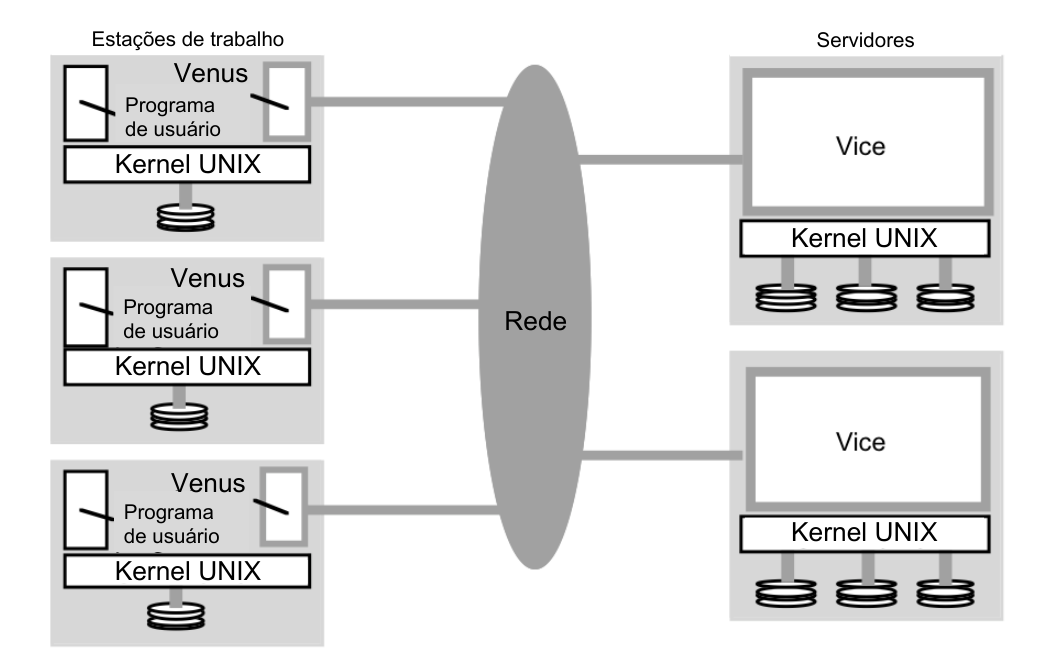
\includegraphics[width=12cm]{arquiteturaAFS.png}
        \caption{Arquitetura do AFS ~\cite{coulouris}}
        \label{fig:arquiteturaAFS}
    \end{figure}
    
    O gerenciamento de cache no cliente é tratado pelo processo Venus, que ao receber uma operação open verifica se o arquivo solicitado já existe na cache e se existe alguma versão mais nova desse arquivo nos servidores. Caso o arquivo da cache esteja defasado a nova versão é solicitada aos servidores e é fornecida ao programa que fez solicitou o arquivo. Quando o arquivo é fechado através da operação \textit{close} o processo Venus (cliente) verifica se o arquivo foi alterado e caso afirmativo envia a nova versão do arquivo ao servidor. É importante ainda ressaltar que o AFS não dispõe de nenhum mecanismo para tratar atualização concorrente de um mesmo arquivo, de forma que se vários clientes enviarem versões diferentes do mesmo arquivo ao servidor, todas exceto a última a ser processada pelo servidor (Vice) serão perdidas sem nenhum aviso ou erro, restando apenas a última requisição processada pelo servidor, que será a versão do arquivo que será salva e estará disponivel ~\cite{coulouris}.
    
    Quanto aos metadados vale citar que os banco de dados ficam replicados integralmente em todos os servidores (Vice) ~\cite{coulouris}, de forma que cada servidor sabe exatamente onde se encontram os arquivos.
    
    Semelhante ao NFS, o AFS só suporta réplica de arquivos para leitura, direcionando todas as escritas nesse arquivo para apenas um servidor, que então faz o sincronismo posteriormente e tem que ser feita de forma explicita ~\cite{coulouris}.
    
    As características citadas acima fornecem ao AFS um bom desempenho para cargas relativamente grandes sem sobrecarregar demasiadamente os servidores, o que fornece grande taxa de escalabilidade, sendo em alguns casos até 60\% mais eficiente no uso de CPU que o NFS com a mesma carga de trabalho ~\cite{coulouris}.
  

    
    %\subsection{\textit{Tahoe-LAFS- Least Authority File System}}
    %Escrever.   
    %\subsection{CODA \textit{Distributed File System}}
    %Escrever.
    %\subsection{\textit{Hadoop File System}}
    %Escrever.
                                            
    \subsection{\textit{Flexible and Adaptable distributed file system} (FlexA)} \label{flexa}
	 
	 O \textit{Flexible and Adaptable distributed file system} (FlexA) ~\cite{silas}, desenvolvido pelo Grupo de Sistemas Paralelos e Distribuídos (GSPD) que é o objeto de estudo desse trabalho, tem foco na utilização de recursos computacionais das estações clientes para diminuir a carga de processamento dos servidores, além de fornecer um sistema de segurança descentralizado e o uso de mecanismo de tolerância a falhas, aproveitando características de diversos SADs, focando em fornecer um SAD com grande escalabilidade ~\cite{silas}.
	
	 O FlexA mudou muito desde sua versão inicial, desenvolvida em 2012 ~\cite{mario}. A versão que será tratada nesse texto é a última versão que ainda está em desenvolvimento, baseada na versão original. Essa versão é o resultado da cooperação de diversos integrantes do GSPD ~\cite{mario}, durante a evolução do sistema nesses dois anos desde sua versão inicial. A arquitetura do sistema original pode ser vista na Figura \ref{fig:arquiteturaFlexaSilas} .
	 
	 \begin{figure}[!ht]
	 \centering
	 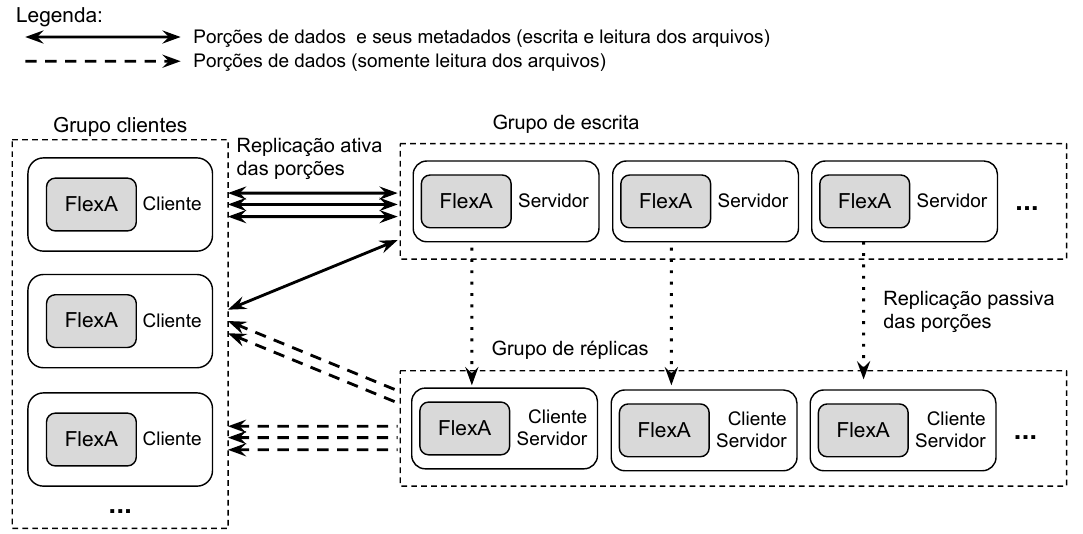
\includegraphics[width=14cm]{arquiteturaFlexAOriginal.png}
	 \caption{Arquitetura original do FlexA ~\cite{silas}.}
	 \label{fig:arquiteturaFlexaSilas}
	 \end{figure}
	 
	 A arquitetura atual do projeto, se baseia muito no que foi proposto por ~\cite{silas} é apresentada na Figura \ref{fig:arquiteturaFlexaMario}.
	 
	 \begin{figure}[!ht]
	 \centering
	 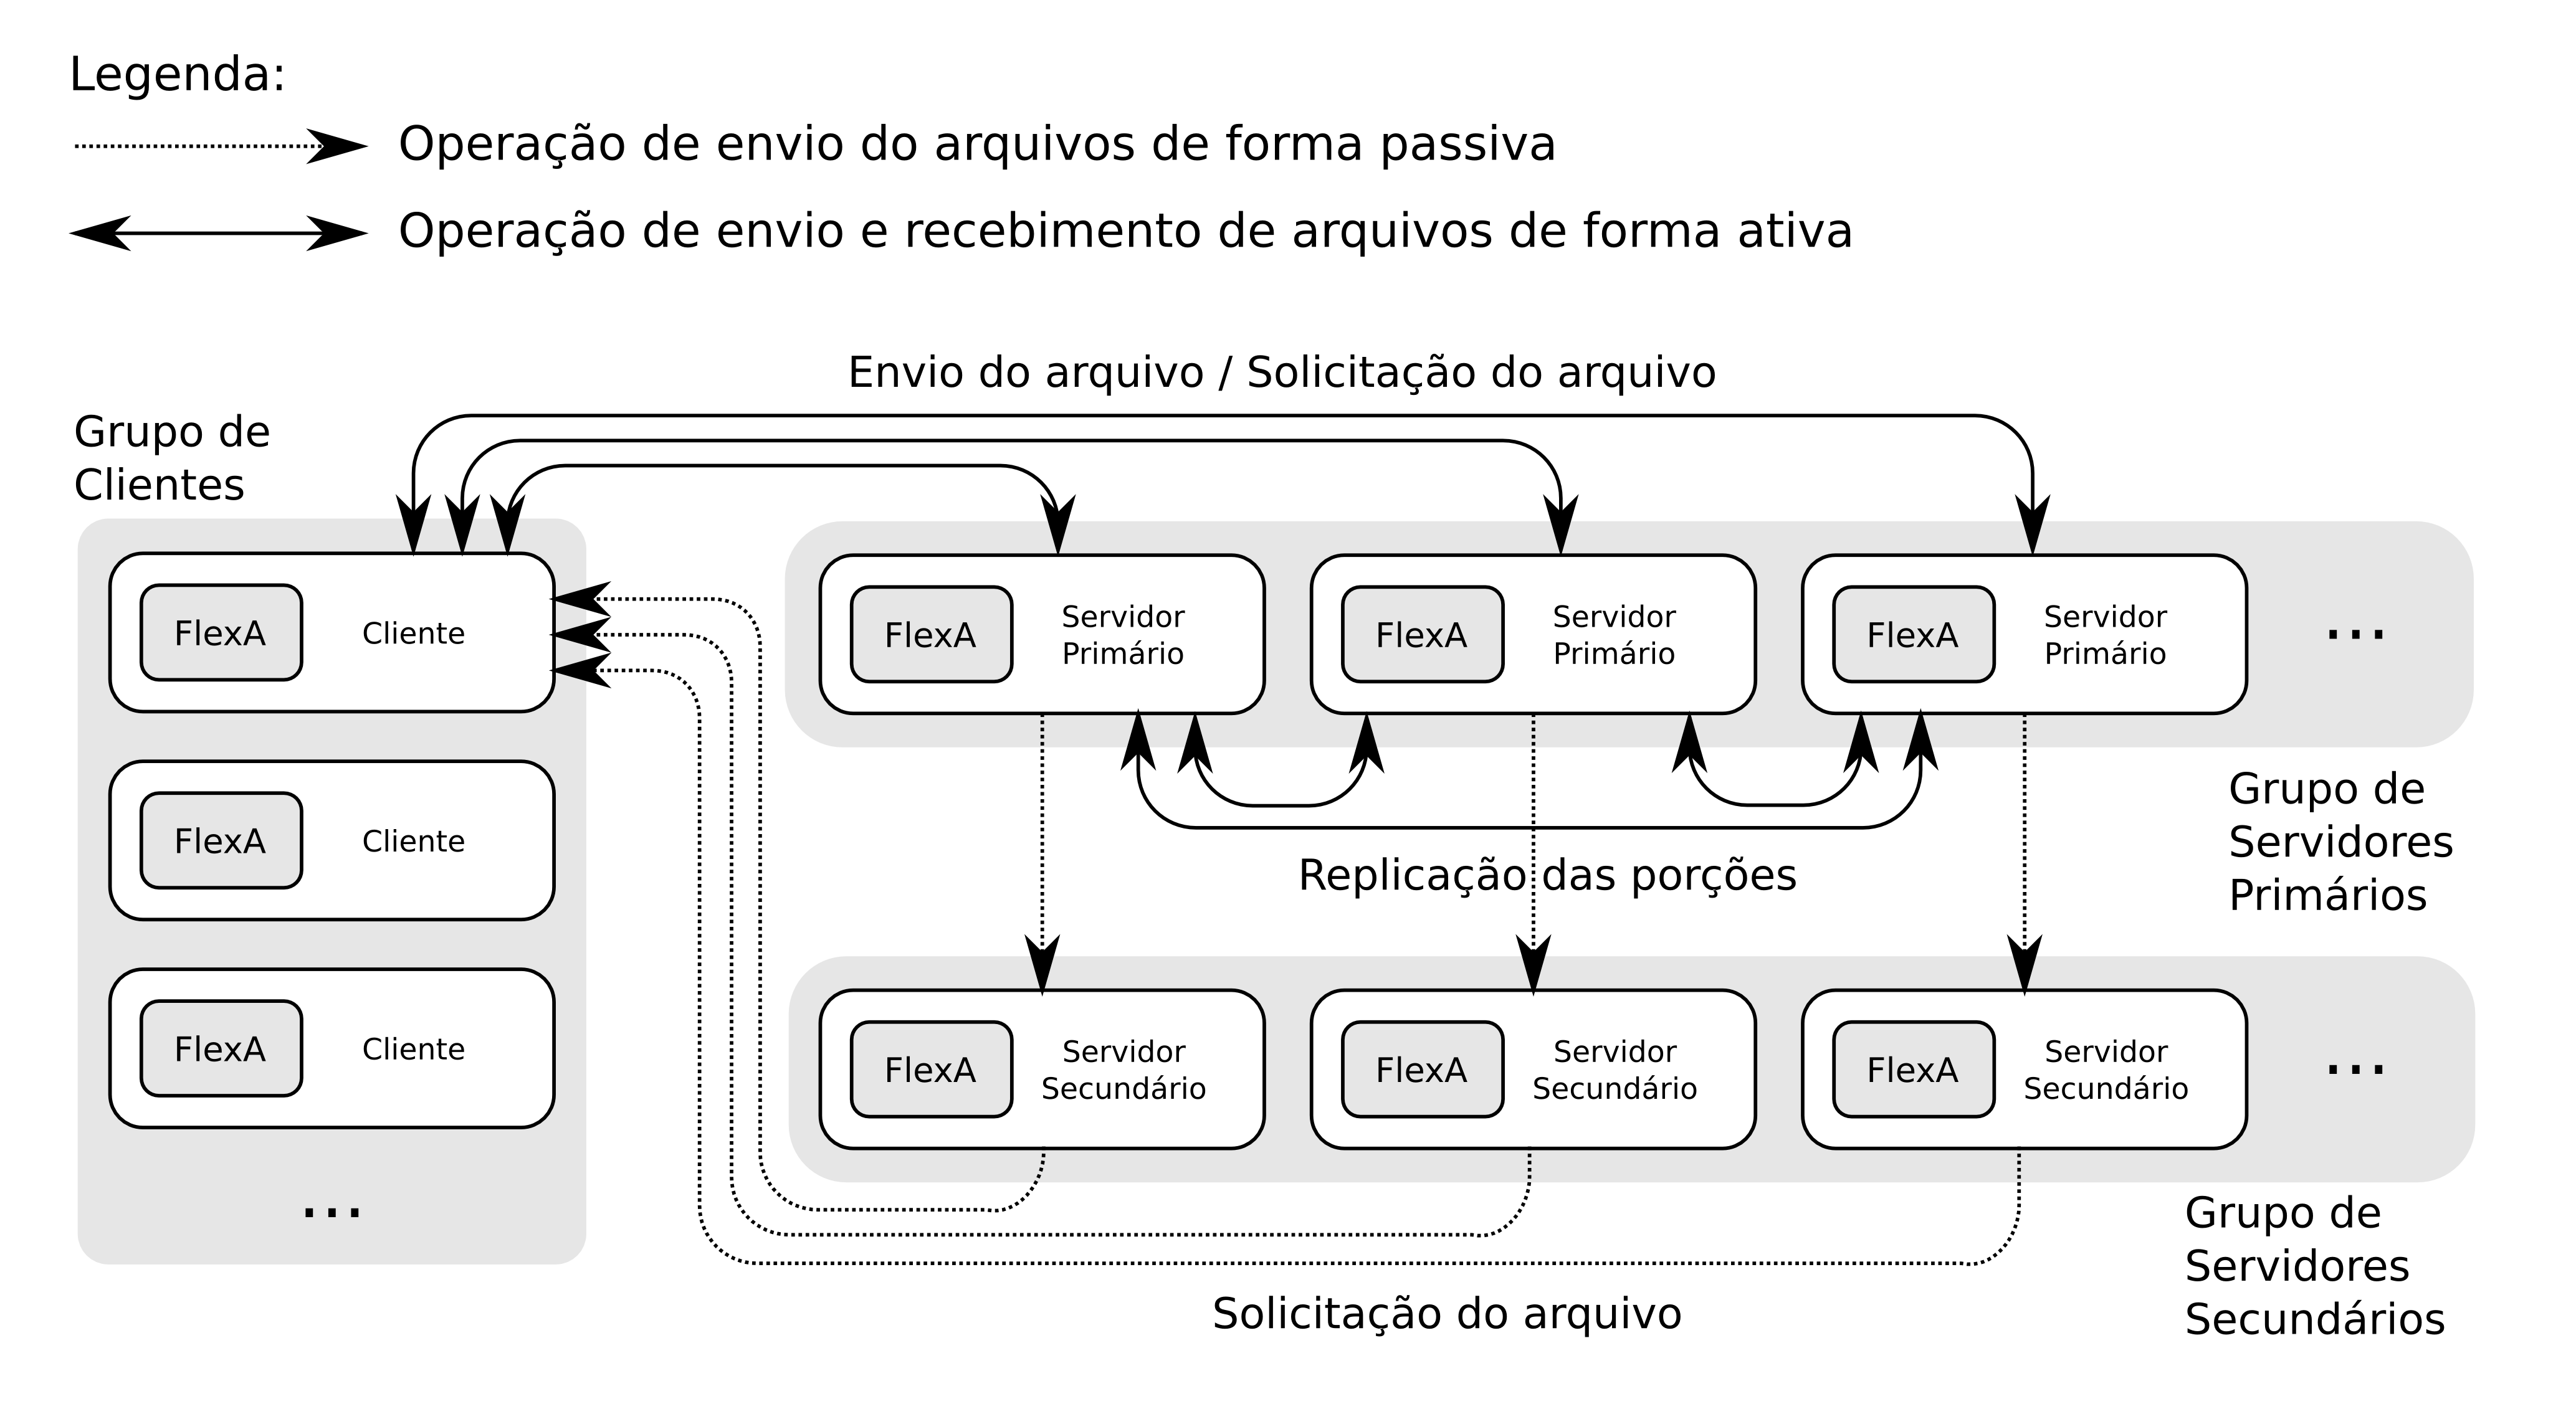
\includegraphics[width=14cm]{arquiteturaFlexA.png}
	 \caption{Arquitetura atual do FlexA ~\cite{mario}.}
	 \label{fig:arquiteturaFlexaMario}
	 \end{figure}
	 
	 Além disso a distribuição dos arquivos também foi alterada, para que o sistema apresente um desempenho melhor do lado cliente, a replicação das porções dos arquivos na fração de 2/3 em cada servidor primário fica agora na responsabilidade dos servidores primários. o diagrama apresentado na figura \ref{fig:arquivosSilas} mostra como era a movimentação dos dados no FlexA original, e a figura \ref{fig:arquivosMario} mostra a nova versão ~\cite{mario}.
	 
	 \begin{figure}[!ht]
	 \centering
	 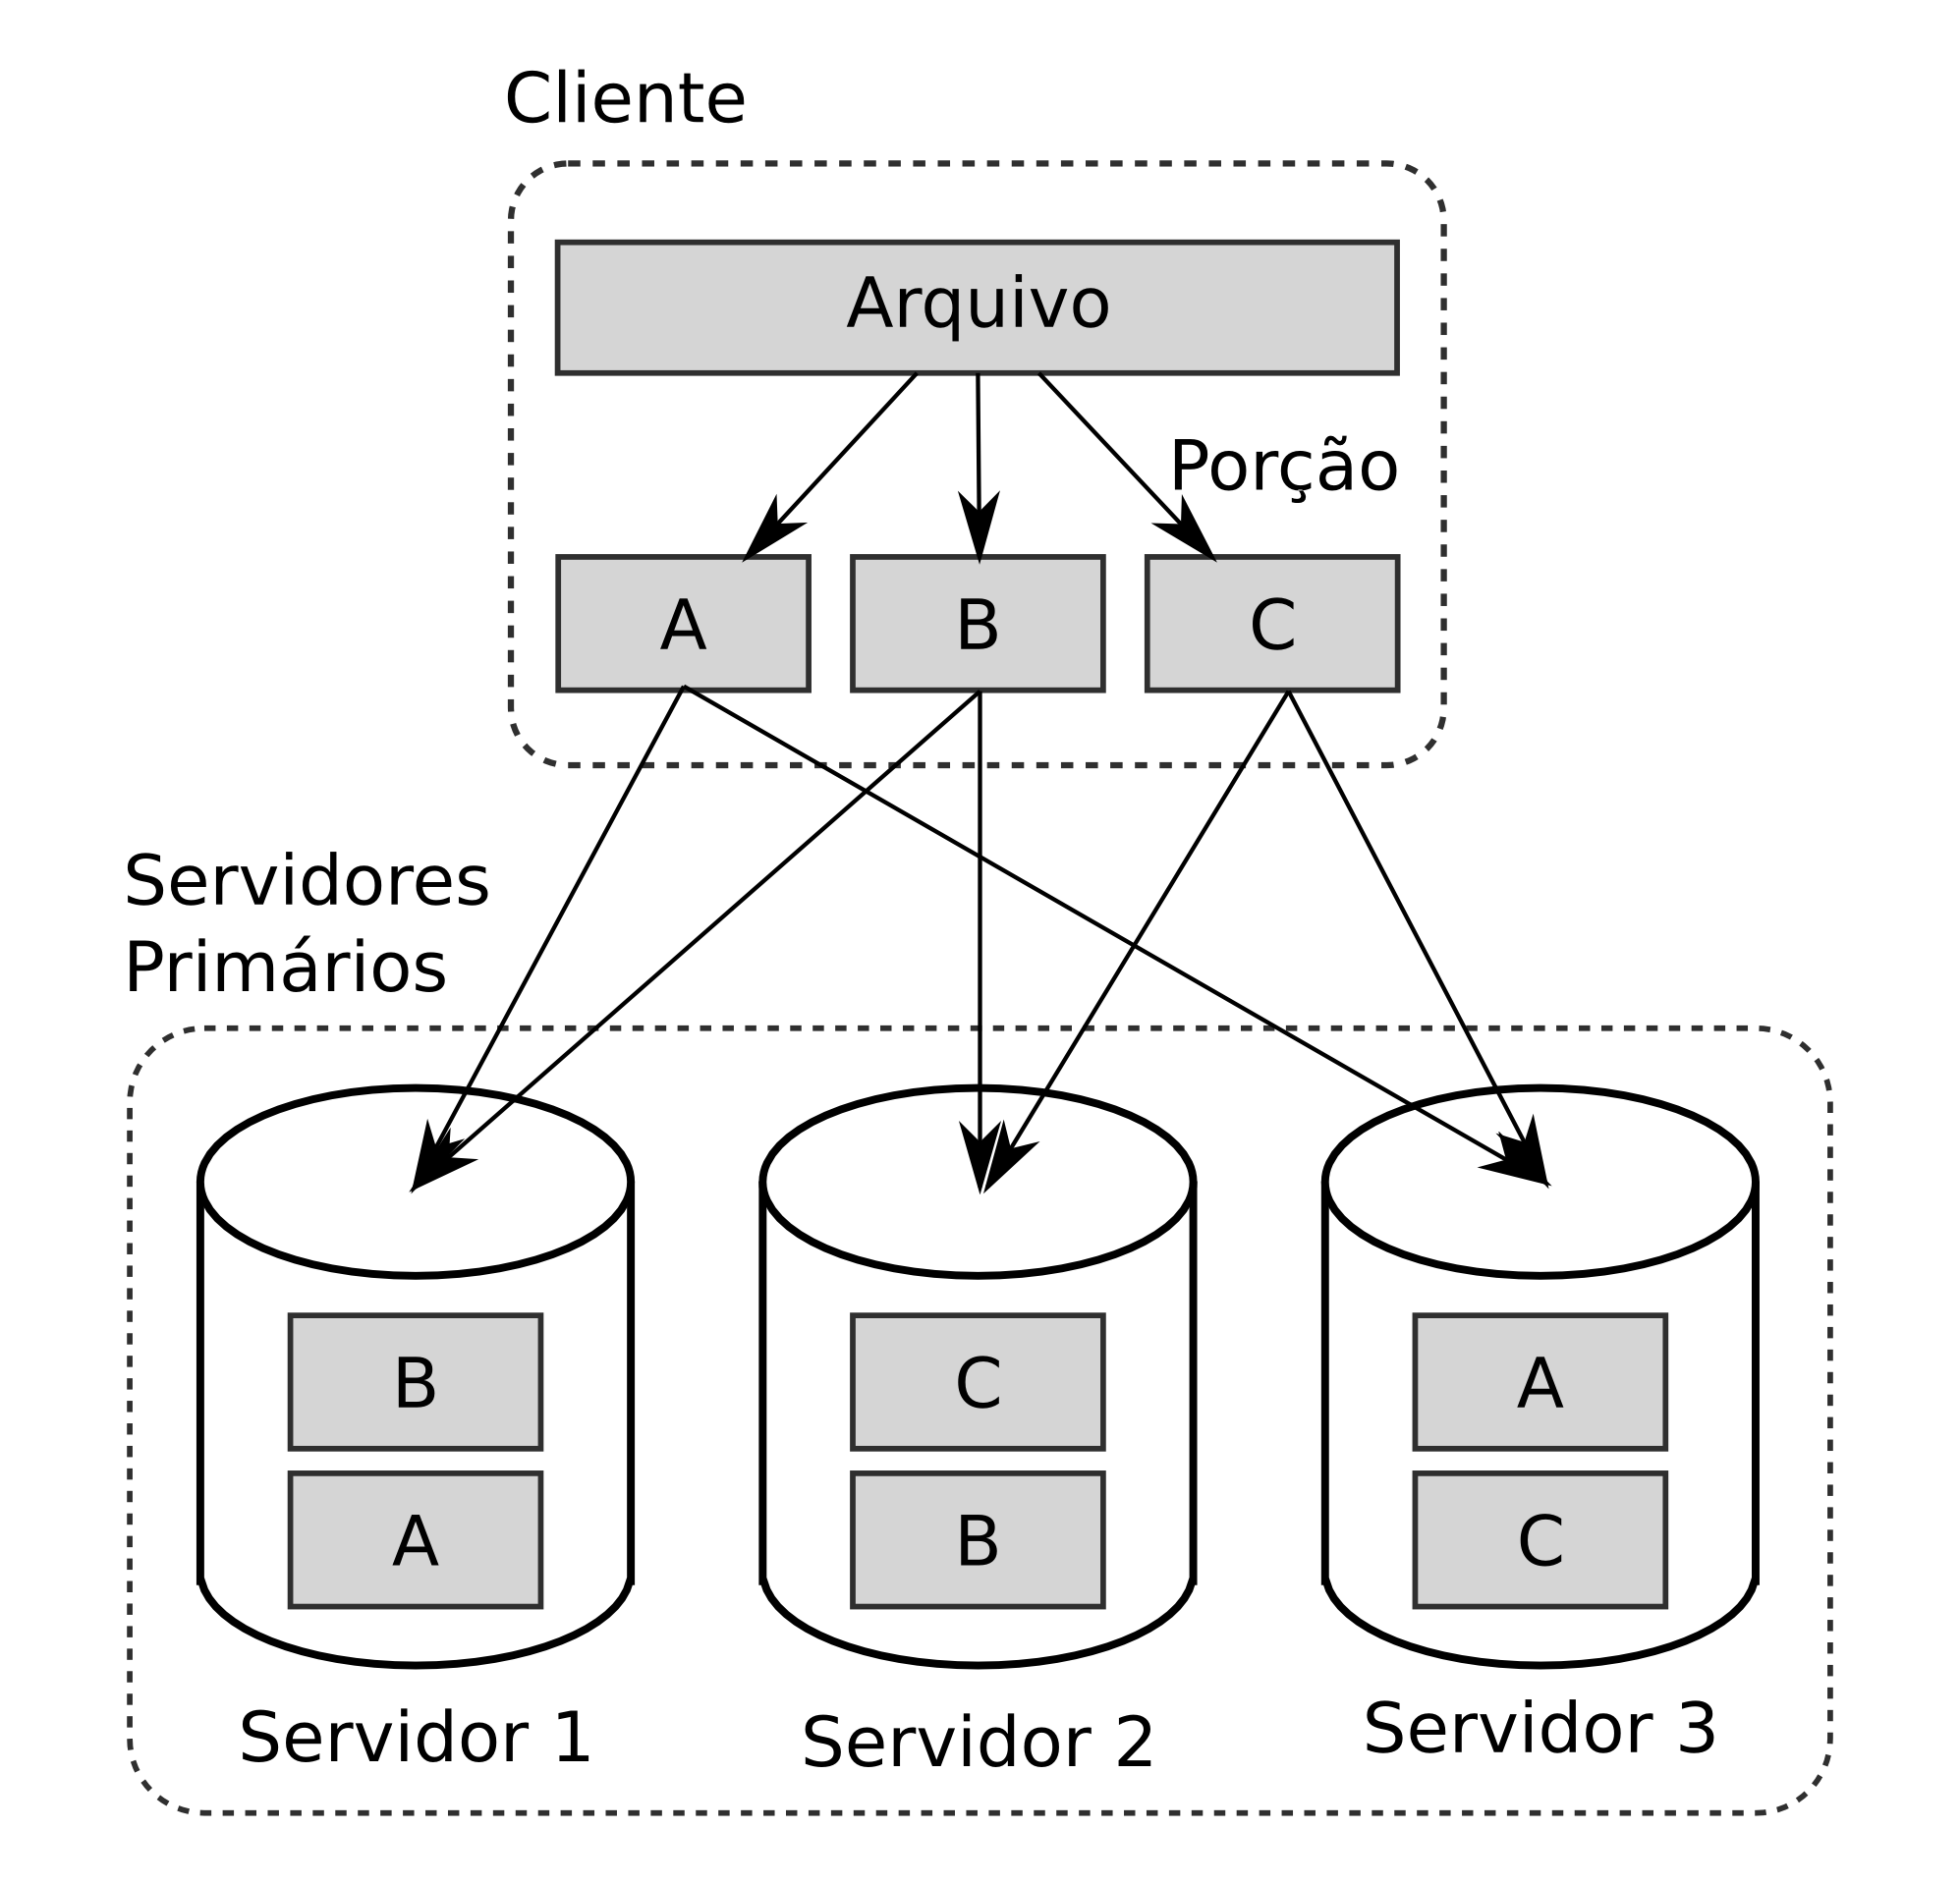
\includegraphics[width=10cm]{arquivosFlexaSilas.png}
	 \caption{Fluxo de dados no FlexA original ~\cite{silas}.}
	 \label{fig:arquivosSilas}
	 \end{figure}
	 
	 \begin{figure}[!ht]
	 \centering
	 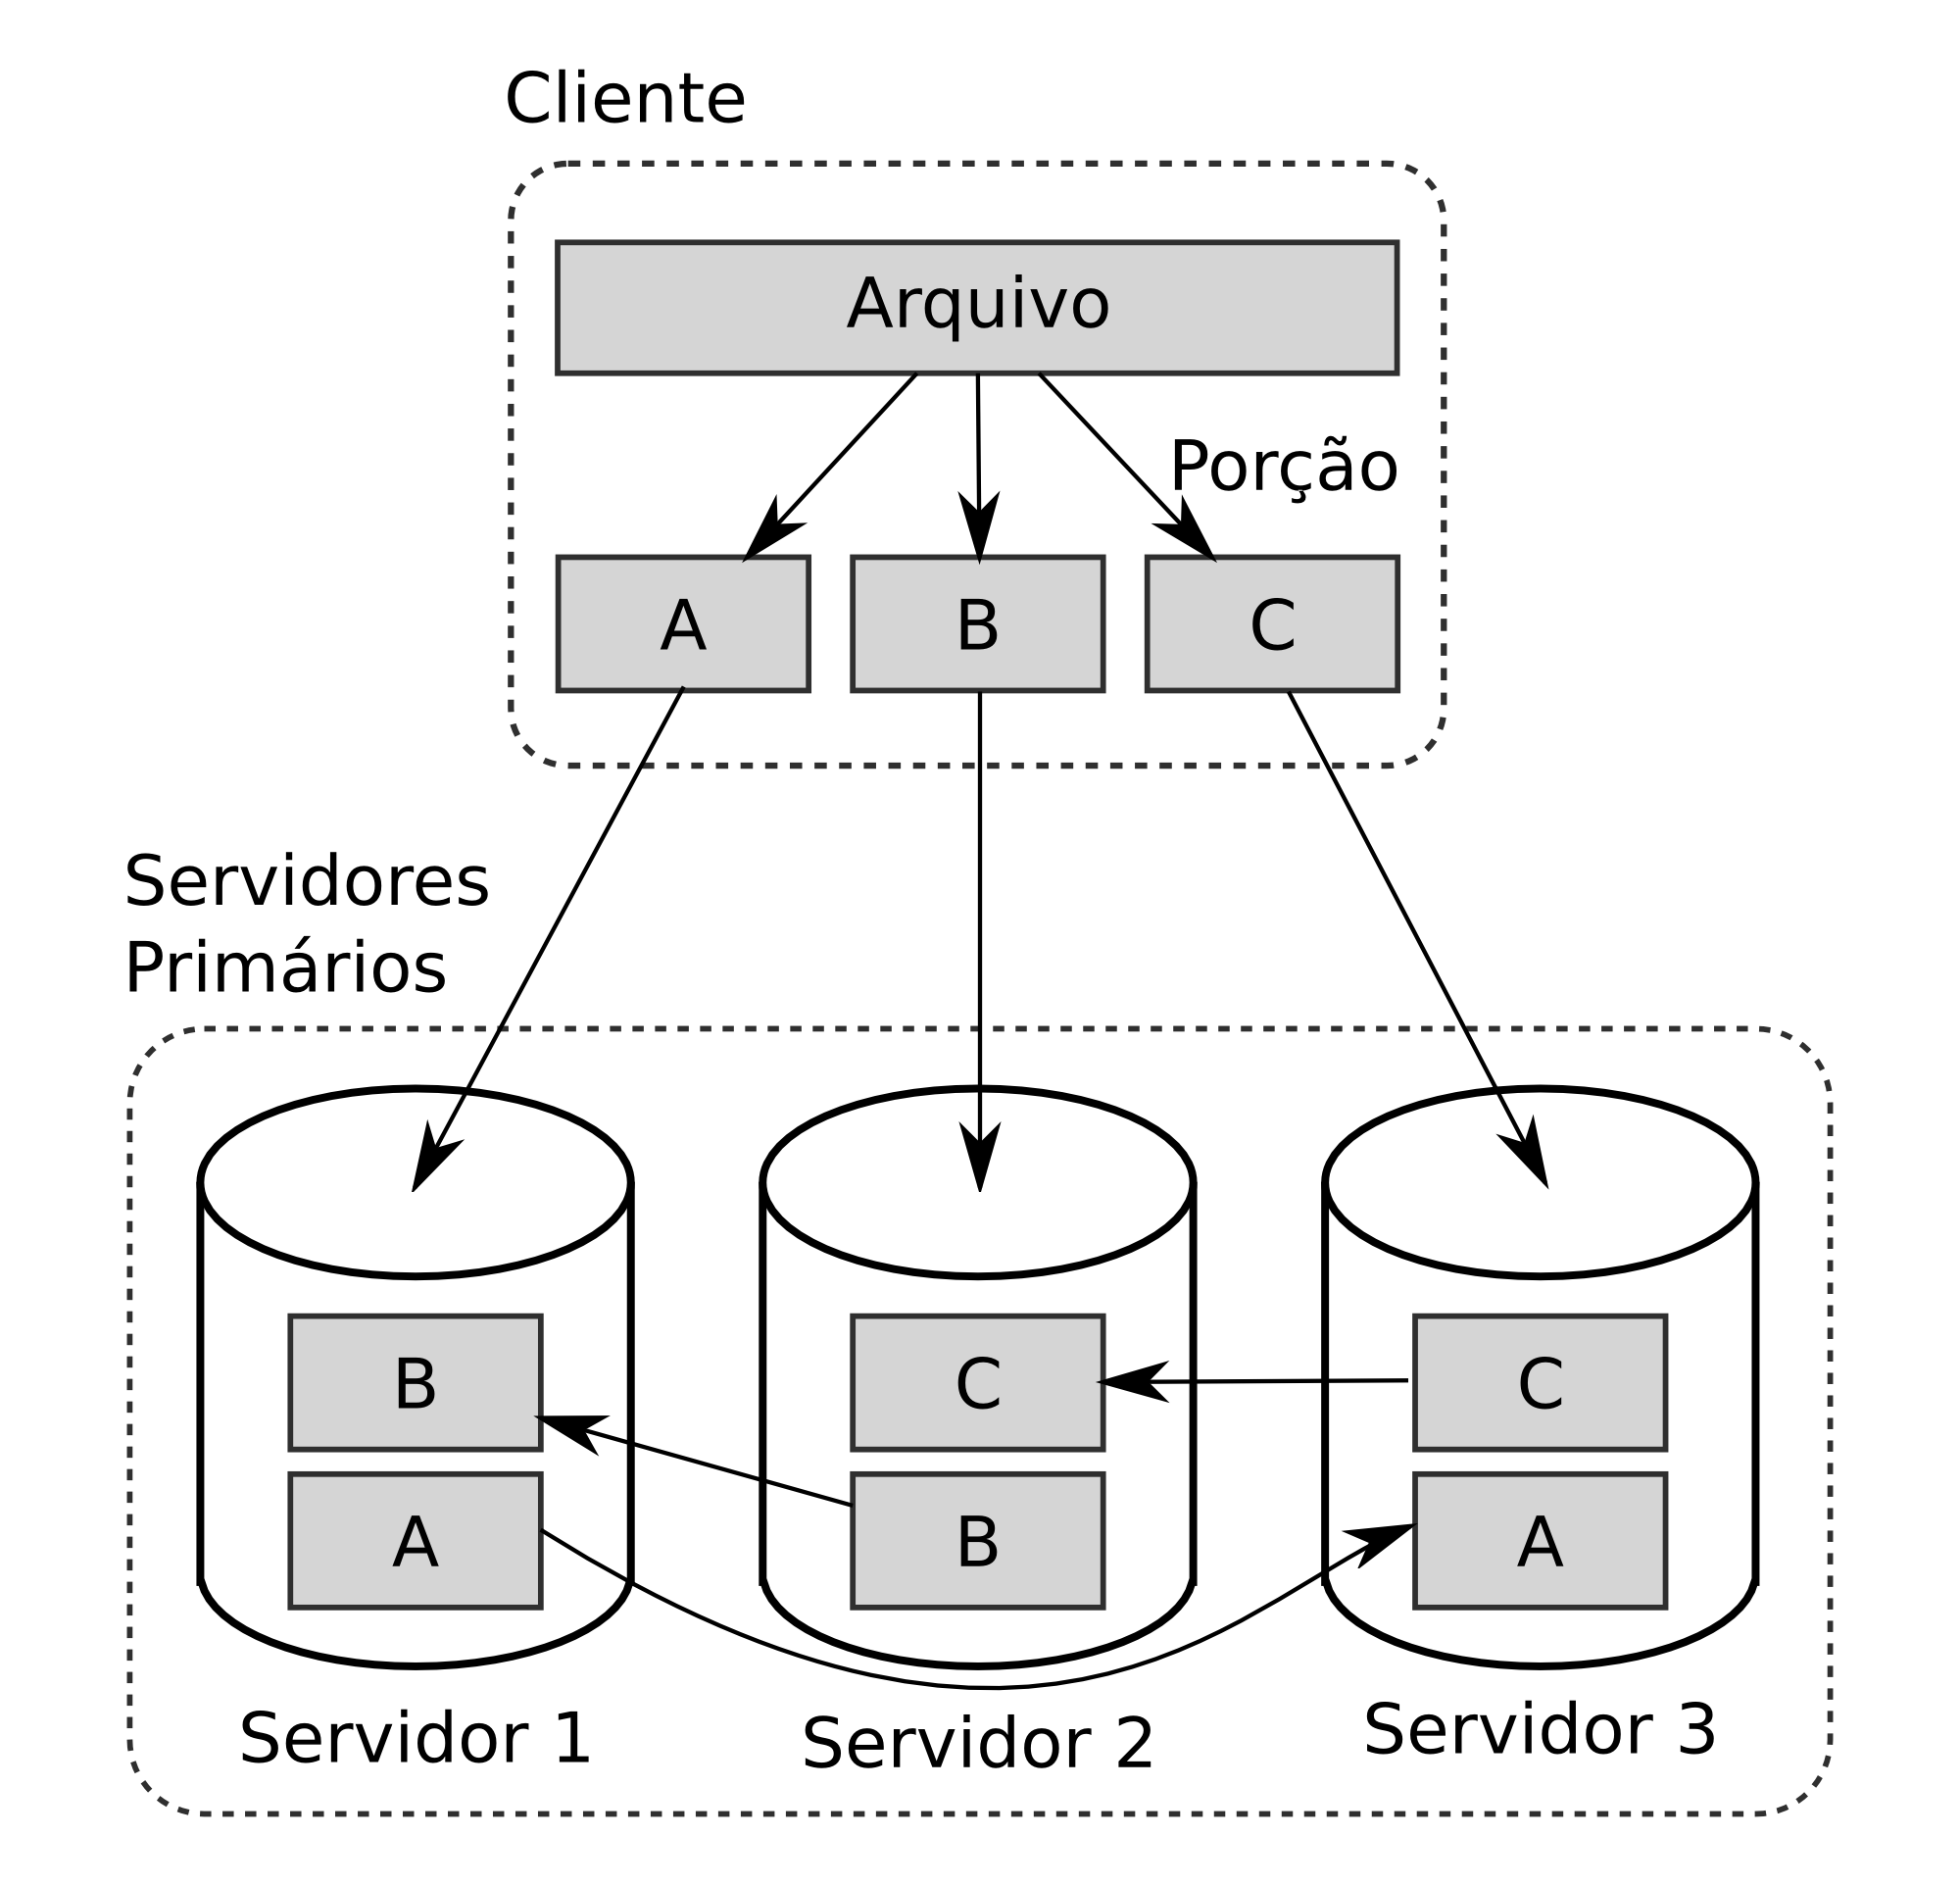
\includegraphics[width=10cm]{arquivosFlexaMario.png}
	 \caption{Fluxo de dados no FlexA atual, elaborado a partir de ~\cite{mario}.}
	 \label{fig:arquivosMario}
	 \end{figure}
	 
	 
	 Para atingir os objetivos descritos acima o FlexA possui diversos mecanismos que serão elencados nas sessões a seguir.
	 
	 \subsection{Segurança}
	    A segurança do sistema é baseada no controle de acesso aos arquivos e também no controle de escrita sobre o mesmo ~\cite{silas}.
	 
    	 \begin{itemize}
    	 
    	    \item Controle de Acesso: é implementado utilizando um trio de chaves para cada arquivo. As chaves que compõe esse trio são:
        	    \begin{itemize}
        	        \item \textit{Verify Key} (VK): fornece acesso ao arquivo, servindo como um identificado único do arquivo no sistema.
        	        \item \textit{Read Key} (RK): é a chave utilizada para cifrar o arquivo. Sem essa chave, mesmo que seja conhecida a VK não é possivel ler o conteúdo do arquivo.
        	        
        	        \item \textit{Write Key} (WK): fornece acesso de escrita no arquivo dentro dos servidores.
        	    \end{itemize}
        	    
            Das três chaves citadas acima a única que não é enviada aos servidores é a chave usada na criptografia do arquivo, a \textit{Read Key}. Dessa forma mesmo que o servidor seja comprometido não é possível obter o conteúdo original dos arquivos que ele armazena ~\cite{mario}.
        	    
        	    
        	    Essas chaves são criadas com base em uma chave privada RSA ~\cite{shamirRSA} especificada pelo usuário, junto com um valor único para cada arquivo chamado de \textit{salt} que é fornecido pelo servidor. Uma vez com a RSA e o \textit{\textit{salt}} o processo feito para obtenção do trio de chaves é o apresentado na Figura \ref{fig:chavesFlexa}.
        	    
        	    \begin{figure}[!ht]
        	    \centering
        	    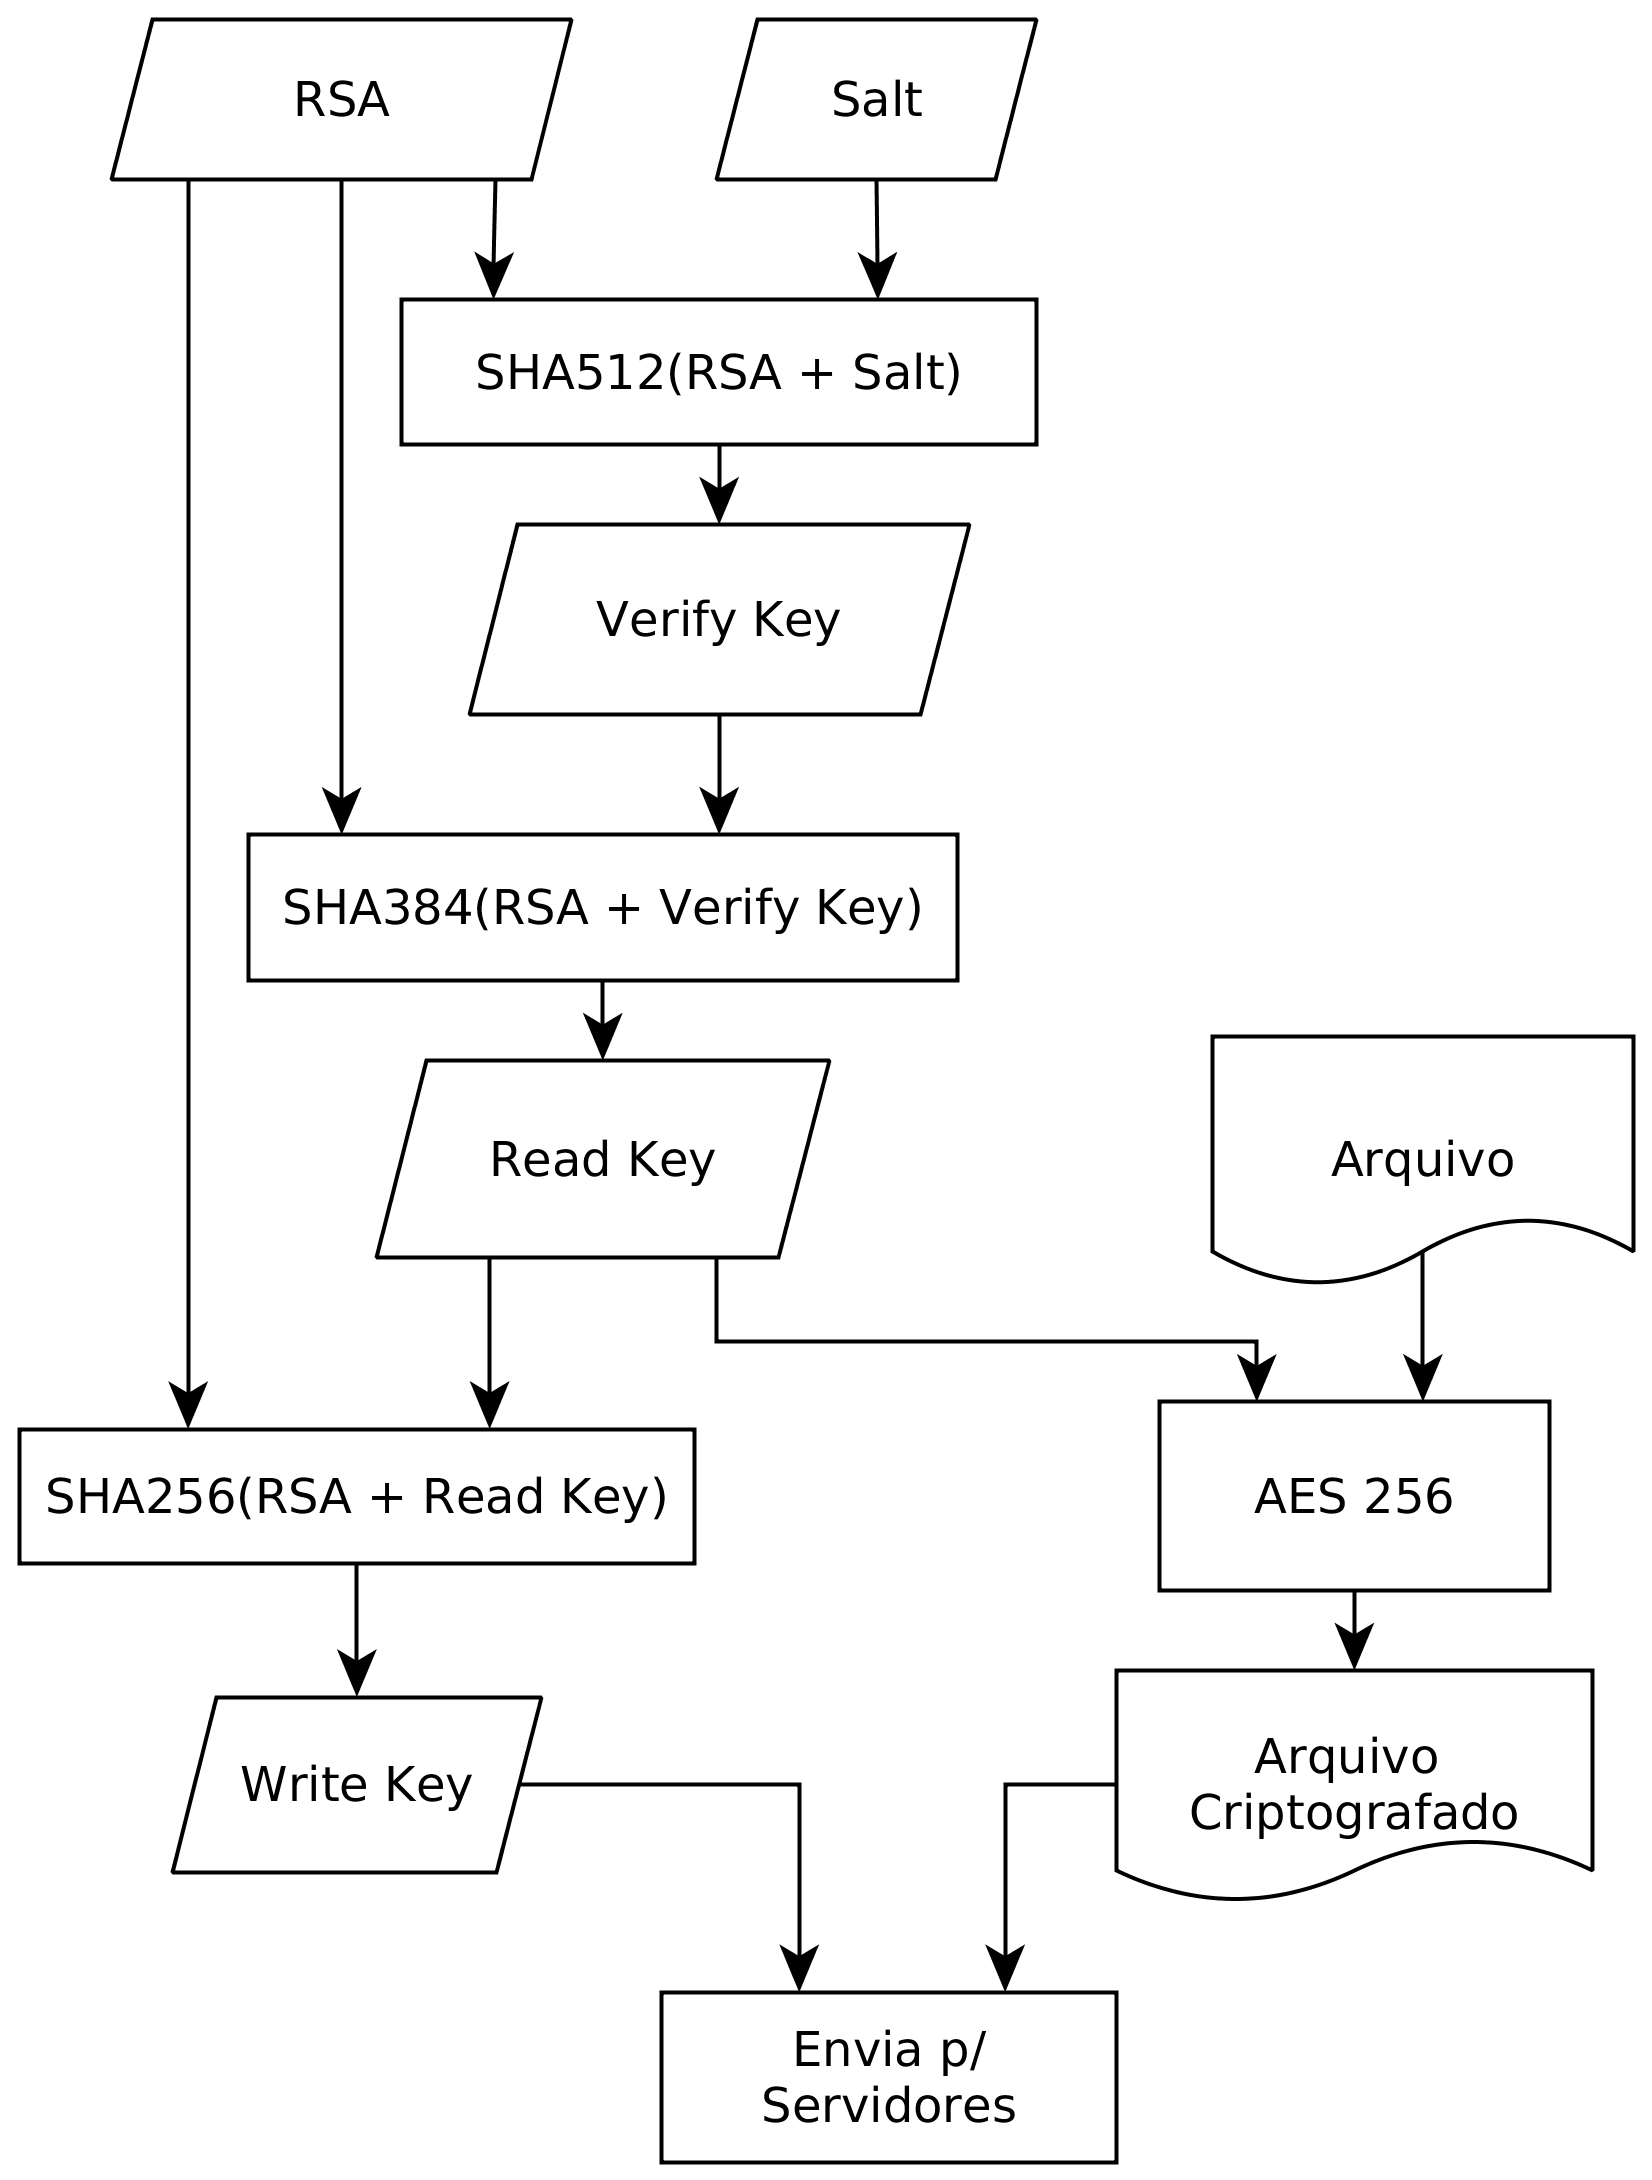
\includegraphics[width=10cm]{chaves.png}
        	    \caption{Diagrama sobre a criação das chaves de acesso e criptografia do FlexA ~\cite{mario}.}
        	    \label{fig:chavesFlexa}
        	    \end{figure}
        	    
        	    Como mostrado na Figura \ref{fig:chavesFlexa} a chave de identificação do arquivo (VK) é gerada utilizando a o \textit{hash} SHA512 da RSA do usuário concatenada com o do \textit{salt} retornado pelo servidor.
        	    Após isso a chave de criptografia (RK) é gerada utilizando a o hash SHA386 da RSA do usuário concatenada com o do identificador do arquivo (\textit{Verify Key});
        	    Por fim é gerado a chave de escrita (WK), utilizando a RSA do usuário concatenada com a chave de leitura.
        	    
        	    Todo o processo criptográfico e de geração de chaves é feito de forma transparente, sem que o usuário tenha que fazer isso de forma manual, notando apenas o tempo que é necessário para fazer a criptografia / descriptografia do arquivo.
    	    
        \item Integridade: O mecanismo de integridade do arquivo é implementado utilizando a chave WK mostrada anteriormente. A permissão de escrita (chave WK) é solicitada sempre que um cliente deseja fazer a operação de escrita (atualização) de um arquivo nos servidores. Dessa forma o cliente deve fornecer a WK correspondente ao arquivo que deseja atualizar, então o servidor comprara a WK fornecida com a armazenada e caso sejam idênticas o servidor faz a substituição do arquivo antigo pelo novo.
        
        Mecanismos para evitar ataques de repetição e outros semelhantes ainda precisam ser implementadas no FlexA, pois a transmissão das chaves de acesso e escrita podem ser facilmente capturadas e reutilizadas com a implementação atual.
        
    \end{itemize}
    
    \subsection{Tolerância a falhas e Adaptabilidade}
        
        Os mecanismos utilizados pelo FlexA para executar esse objetivo são o uso de réplicas das porções dos arquivos, que são enviados para diversos servidores e lá são replicados com o grupo de servidores secundários. Também é utilizada a possibilidade de um servidor secundário assumir além da sua função a de um servidor primário caso seja necessário por falha de algum primário ou sobrecarga do grupo de servidores primários ~\cite{mario}.
        
        Sempre que um servidor primário ou secundário falha, é executado um processo que faz o sincronismo do servidor com os outros servidores ativos para que esse assuma o estado atual do sistema e volte o mais breve possível a colaborar com o atendimento dos clientes ~\cite{silas}.
        
    
    \subsection{Escalabilidade}
    
        Os principais fatores que auxiliam na escalabilidade do sistema são:
        
        \begin{itemize}
            \item Criptografia e descriptografia dos arquivos nos clientes: Evitam o consumo de UCP nos servidores, deixando-os mais disponíveis para atender a novas requisições.
            \item Divisão dos arquivos em diversas porções nos clientes: Diminuem o uso de armazenamento e uso dos discos dos servidores.
            \item União das diversas porções que compõe um arquivo nos clientes: Também influenciam no uso de disco dos servidores, liberando os discos para atenderem outras requisições mais rapidamente.
            \item Leitura e escrita das porções dos arquivos de diferentes servidores, evitam sobrecarregar o uso de banda de apenas um servidor e aumentam o uso da banda no cliente.
            \item Utilização agressiva de cache nos clientes: Essa técnica evita acessos recorrentes aos servidores, principalmente para arquivos que são pouco atualizado ou são utilizados por apenas um usuário.
            \item Uso de sistemas de replicação para servidores secundários: Auxiliam nas operações de leitura dos arquivos pelos clientes.
        \end{itemize}
        
        
    \subsection{Flexibilidade}
    
        Como boa parte da carga de processamento e uso do disco no FlexA é transferida aos clientes, o sistema pode operar com \textit{hardware} de baixo custo sem grandes problemas. Isso ainda fornece ao FlexA a possibilidade de que caso seja necessário clientes com mais recursos disponíveis podem passar a fazer parte do grupo de servidores auxiliando no atendimento a requisições de outros clientes. Essa característica faz com que o sistema aproveite muito recurso que estaria ocioso em sua rede, principalmente em momentos de uso intensivo dos servidores ~\cite{silas}.
        
        Além disso o sistema é projetado para que seja possível fazer a troca dos mecanismos de segurança, regras de gerenciamento da cache nos clientes,  métricas de divisão das porções e diversos outros elementos do sistema de forma simples, principalmente devido a escolha do Python como linguagem de programação, facilita o acesso ao código fonte do FlexA ~\cite{silas}.
        
    \subsection{Abertura}
    
    A abertura do FlexA é dada basicamente pelo fato de o sistema ter o código fonte aberto e disponível ~\cite{silas}, sendo necessário aprimorar a documentação existente. 


\section{Chamada de Procedimentos Remotos (RPC)}

    Para realizar comunicação entre cliente e servidores é possível utilizar diversas técnicas diferentes. Nesse trabalho a Chamada de Procedimento Remoto ou \textit{Remote Procedure Call} (RPC) é uma ferramenta muito utilizada pois é a partir dela que a maior parte das comunicações entre cliente e servidor acontecem. A escolha desse paradigma foi feita pela simplicidade do projeto e desenvolvimento. 
    
    O RPC utiliza um paradigma de comunicação de alto nível, ocultando do desenvolvedor quase todo o processo de estabelecimento de conexão, transmissão dos dados, conversão dos dados e bloqueio do cliente ~\cite{rpc} ao realizar requisições.
    
    A descrição básica da comunicação via RPC é feita em ~\cite{rpc}. Para a utilização do RPC na implementação de um serviço é necessário um processo chamado de servidor RPC (Servidor) que possui as funções disponíveis que serão solicitadas por um cliente através de uma requisição RPC. Assim cabe ao Servidor registrar todas as funções que o cliente pode requisitar. Após registrar as operações o Servidor inicia a escuta por requisições.
    
    Em outro \textit{host}, um processo chamado Cliente faz uma Requisição RPC ao Servidor. O Servidor executa a função solicitada, com os parâmetros enviados e retorna o resultado ao cliente.
    
    De acordo com ~\cite{rpc} o uso de RPC reduz em média 50\% da complexidade no desenvolvimento da comunicação entre cliente e servidor.
    
    \subsection{XML-RPC}
    
    No mercado existem diversas soluções para o uso de RPC. O XML-RPC é uma implementação de RPC que utiliza TPC/IP junto com HTTP e XML para a troca de mensagens entre servidor e cliente ~\cite{xmlrpc}. O uso de um padrão como o XML-RPC é também justificado pela representação dos dados que é mantida através de diversas arquiteturas ~\cite{xmlrpcMessage}
    
    A versão atual do FlexA utiliza o XML-RPC para todas as comunicações entre cliente/servidor exceto para a transmissão de arquivos ~\cite{mario}. A transmissão dos arquivos é feita via \textit{socket} para evitar o processo de \textit{marshalling} dos arquivos que tende a ser demasiadamente custoso em questões de uso de UCP e demorado, dessa forma reduzindo o tempo de entrega dos arquivos ao cliente.
    
    Um diagrama bem simples sobre o funcionamento desse paradigma descrito acima é exibido na Figura \ref{fig:xmlrpc}.
    
    \begin{figure}[!ht]
    \centering
    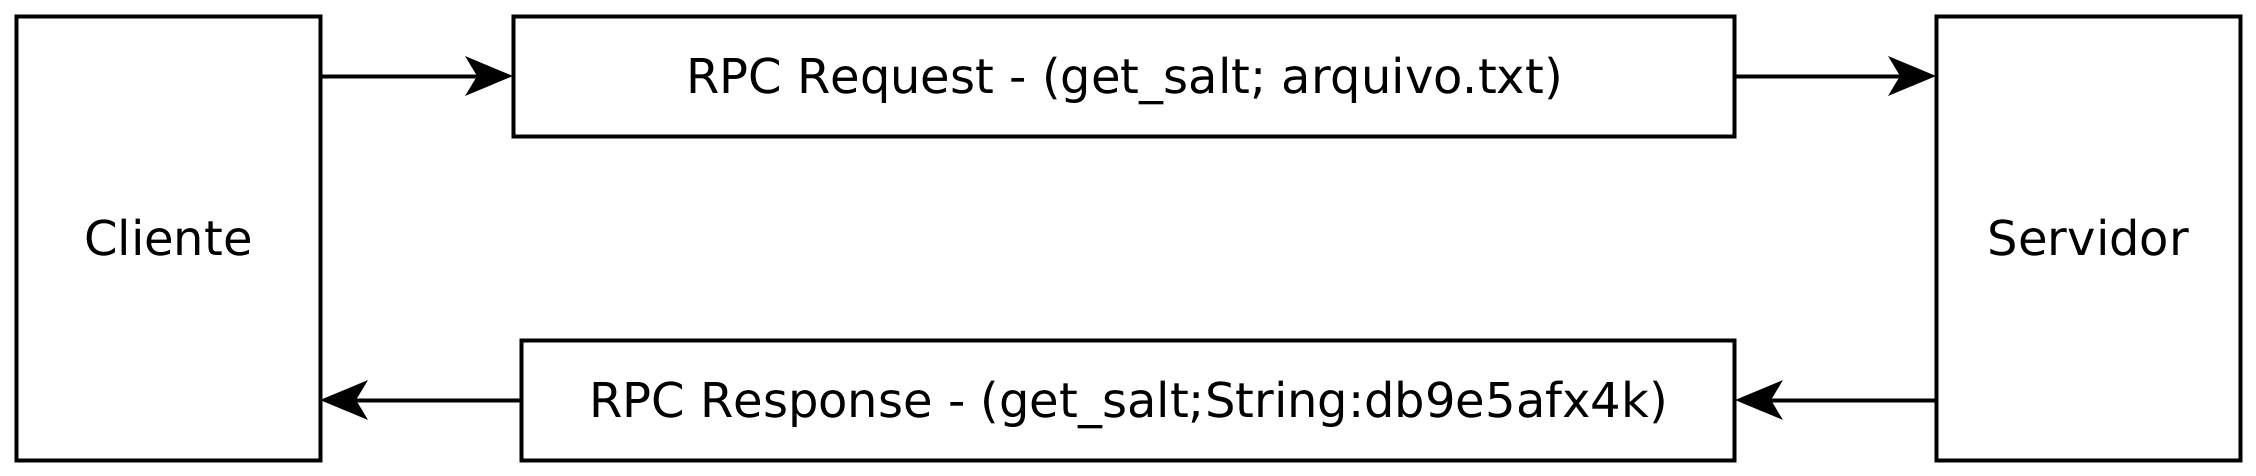
\includegraphics[width=10cm]{xmlrpc.png}
    \caption{Diagrama que exibe a comunicação via XML-RPC. ~\cite{xmlrpc} (Adaptado)}
    \label{fig:xmlrpc}
    \end{figure}
    
    Como pode ser visto na \ref{fig:xmlrpc}, o cliente faz a requisição de uma função remota, passando os parâmetros. Toda a comunicação é feita com o uso de XML. O servidor recebe a requisição, processa e retorna o resultado também em XML. Um outro exemplo mostra como é feita a comunicação de uma requisição com XML-RPC como pode ser visto na Figura ~\ref{fig:xmlrpcMessage} . O processo de resposta da requisição segue o mesmo principio.
    
    \begin{figure}[!ht]
    \centering
    \fbox{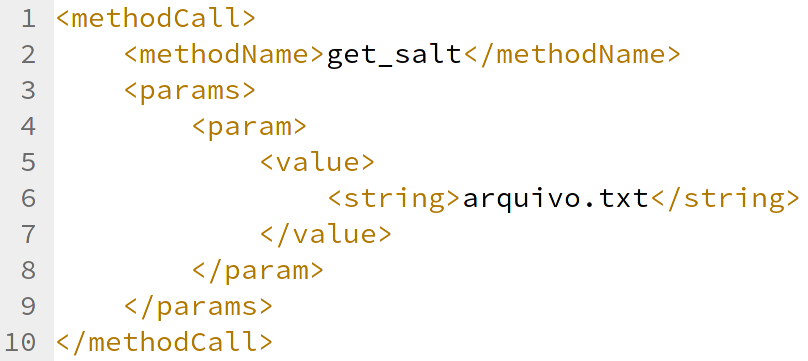
\includegraphics[width=10cm]{xmlrpcMessage.png}}
    \caption{Exemplo de mensagem XML utilizada na chamada de procedimentos remotos com XML-RPC.}
    \label{fig:xmlrpcMessage}
    \end{figure}


\section{Dispositivos Móveis}

    Quanto a classificação de dispositivos móveis, é muito difícil fornecer uma definição formal que seja adequada. Assim essa definição pode ser feita em duas partes, como feita em ~\cite{mobileDevices}.
    
    \subsection{Dispositivos Móveis}
    De acordo com ~\cite{mobileDevices}, dispositivos móveis são dispositivos portáveis como    \textit{laptops}, \textit{Personal Digital Assistants} (PDA), \textit{tablets}, \textit{smart phones}, \textit{handhelds}, \textit{MP3 Players}, consoles de jogos portáteis entre outros. Variando de dispositivos com pouquíssima autonomia, baixa ou nula conectividade e pouca capacidade computacional até dispositivos de ultima geração com autonomia relativamente alta (algumas dezenas de horas de uso constante), potência computacional muitas vezes superior a computadores de mesa e \textit{notebooks} e grande conectividade utilizando diversas tecnologias diferentes. 
    
    
    \subsection{Computação Móvel}
    Dentro do escopo desse trabalho mais importante que a definição de dispositivos móveis é a definição  computação móvel, que é apresentada por ~\cite{mobileDevices} como sendo um conjunto de dispositivos móveis que fornecem ao usuário um sistema computacional que pode operar em dois modos: conectado e desconectado. Quando desconectado de redes de dados esses dispositivos devem funcionar de forma dessincronizada com sua fonte de dados, e quando conectados novamente a redes que fornecem acesso a transmissão de dados devem fazer o sincronismo dos dados através de operações de \textit{upload/download}.
    
    
\section{Android}

Na maioria das vezes é necessário um sistema operacional (SO) que gerencie um dispositivo móvel, esse sistema operacional pode ser o Android ~\cite{android} ou outro sistema operacional comum ou preferencialmente próprio para dispositivos desse tipo. Existem atualmente no mercado dezenas de SOs diferentes para dispositivos móveis, mas os que mais se destacam frente aos usuários e grandes fabricantes são Android (\textit{Open Handheld Alliance}) e iOS (Apple) ~\cite{mobileDevicesMarketShare}.

Mais do que um simples sistema operacional, o Android é composto por diversas camadas de software (~\textit{Android Software Stack}) que fornecem ao sistema suporte a uma grande variedade de dispositivos e flexibilidade no seu uso ~\cite{android}. Essas camadas são exibidas na Figura \ref{fig:androidStack}.

\begin{figure}[h]
\centering
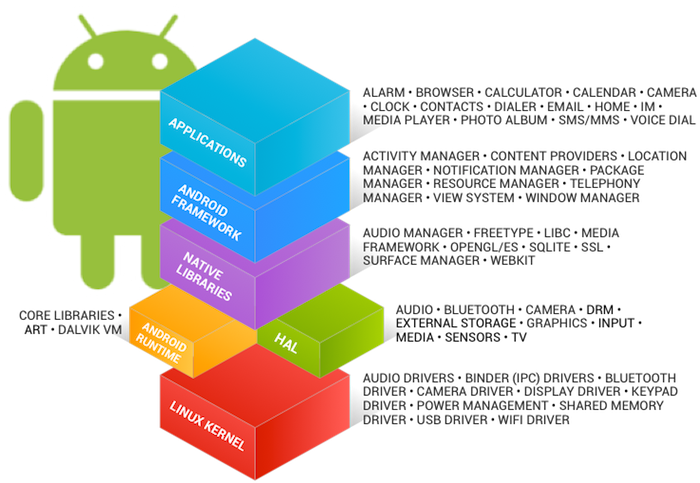
\includegraphics[width=14cm]{androidStack.png}
\caption{Camadas de software que compõe o sistema Android ~\cite{android}.}
\label{fig:androidStack}
\end{figure}


% Ideia desse capitulo: Apresentar o desenvolvimento do projeto-

%% Revisado por Gabriel Saraiva
%% Revisado por Renata

% Restrições do projeto atual         OK
% Propostas de melhorias                OK
% Documentação do Projeto               OK
% Adaptação do servidor python          OK
% Implementação do cliente Android      OK

\chapter{Descrição e desenvolvimento do projeto}
\label{cap3}

    Neste capítulo são apresentados o desenvolvimento da proposta do projeto e também sua implementação no FlexA. Inicialmente serão abordados as restrições encontradas no projeto atual e a motivação para corrigi-las. Então será apresentada a documentação desenvolvida para que o projeto possa ser viável a longo prazo, então serão detalhadas as adaptações realizadas no módulo servidor para que esse passe a ser compatível com a nova especificação. Por fim, com o novo servidor pronto, será apresentada a implementação do cliente para Android.
    
    %% Para não avacalhar com o projeto do Mario (rsrsrs eu ri disso)... O termo é muito engraçado. Não fiz por mal =)
    
    \section{Restrições da versão atual do FlexA}
    
        A versão atual do FlexA, ainda em um estágio inicial de desenvolvimento, carece de um modelo de programação bem definido, sua documentação precisa ser aprofundada e não menos importante de um protocolo de comunicação precisa ser bem explicitado.
        
        Os principais pontos que serão abordados nesse projeto serão:
        
        \begin{itemize}
            \item Documentação documentação inicial do projeto, como um diagrama de classes, casos de uso e também um diagrama com os módulos do sistema e como eles se integram.
            \item Formalização do protocolo de comunicação.
            \item Adaptação incremental do módulo servidor para que ele passe a ser compatível com a documentação gerada.
            \item Implementação do módulo cliente para Android.
        \end{itemize}
        
        A motivação para essas melhorias é que elas fornecerão uma base sólida para que no futuro possam ser incorporados no projeto atual os resultados de trabalhos já realizados em versões anteriores do FlexA, que são listados pelos títulos:
        
        \begin{itemize}
            \item Detecção de Falhas de Comunicação e Balanceamento de Carga no FlexA ~\cite{danilo};
            \item Metodologia para Recuperação de Falhas e Garantia de Disponibilidade no FlexA ~\cite{thiago};
            \item Implementação e avaliação de desempenho de algoritmo de criptografia em GPU para o FlexA ~\cite{leandro};
            \item Sincronização, consistência e falhas no FlexA ~\cite{matheus};
            \item Disponibilidade em um sistema de arquivos distribuído flexível e adaptável ~\cite{lucio};
        \end{itemize}
        
       
    Além de tornar mais fácil a incorporação dos resultados obtidos com os trabalhos citados, a nova documentação deve tornar o sistema fácil de se manter e evoluir e permitir que diversas equipes colaborem com o trabalho de forma simultânea.
    
    
        
    \section{Documentação do projeto}
        
    Um estudo a fundo do sistema foi feito, utilizando a documentação que existia e a análise do código-fonte, para entender o funcionamento e comportamento do sistema e também como era definida a estrutura atual do projeto. 
    
    \subsection{Módulos do Sistema}
    
        Para representar o sistema de forma mais abstrata foi criado um diagrama dos módulos do sistema atual, e suas dependências conforme pode ser visto na Figura \ref{fig:pacotesMario}.
        
        \begin{figure}[!ht]
            \centering
            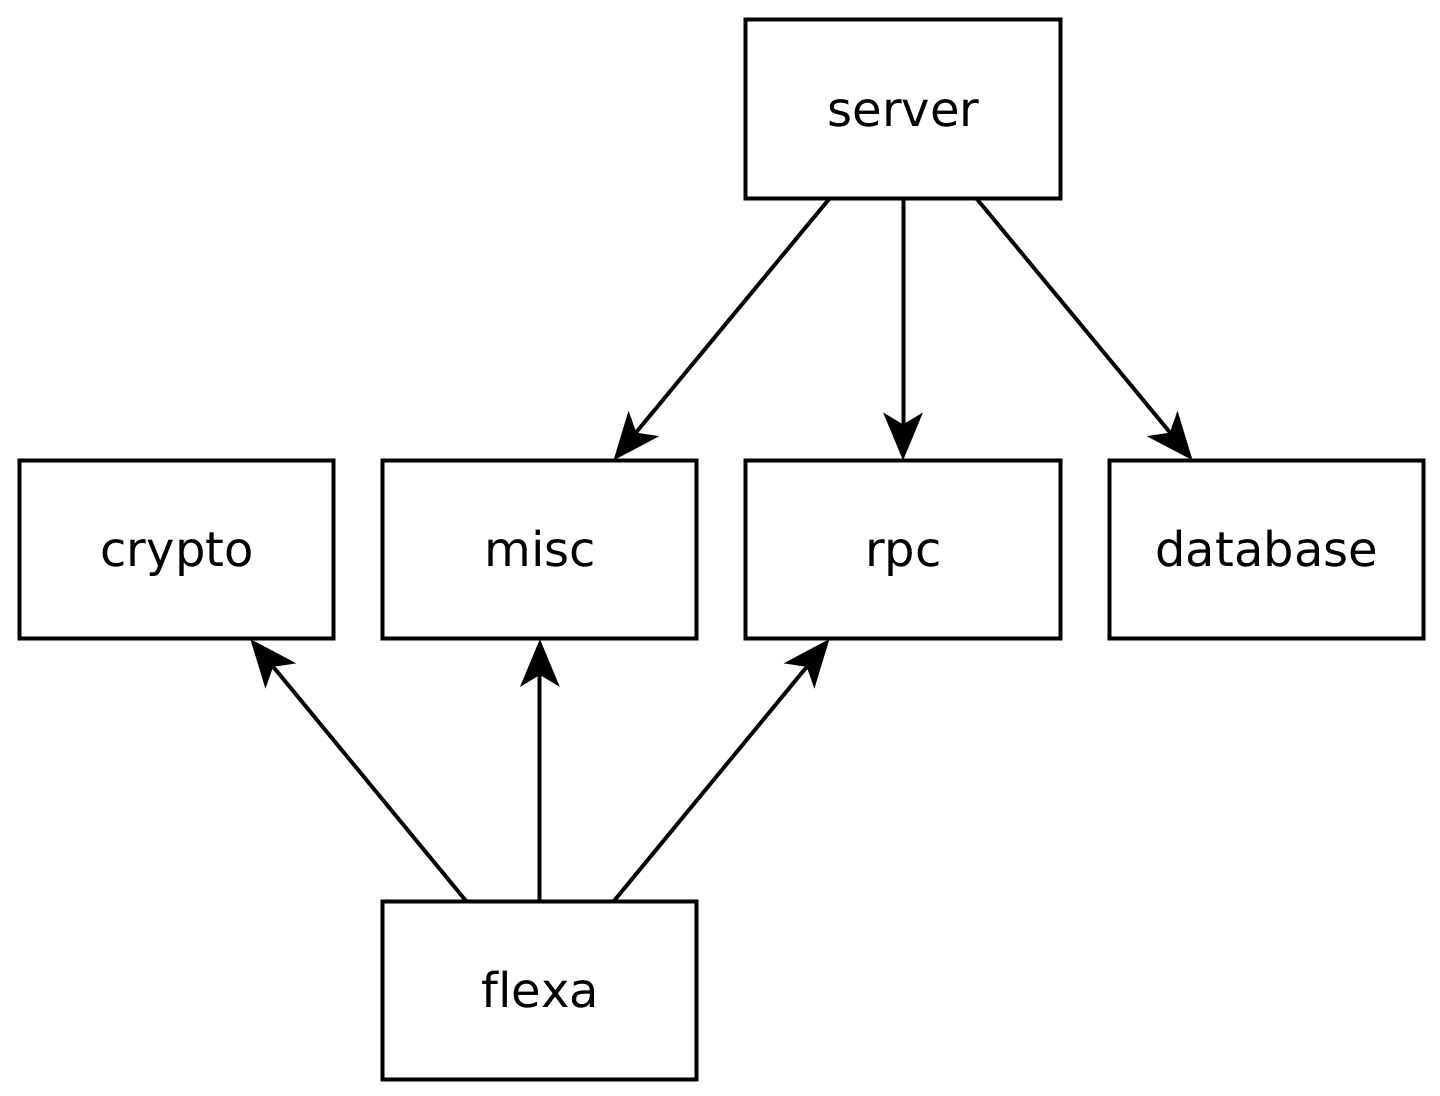
\includegraphics[width=10cm]{pacotesMario.png}
            \caption{Módulos do sistema atual e suas dependências. Criado com base no código fonte do projeto ~\cite{mario}.}
            \label{fig:pacotesMario}
        \end{figure}
        
        Esse diagrama foi gerado a partir do estudo do código-fonte da versão atual do projeto. Apenas por esse diagrama já é possível notar que o módulo Servidor não utiliza os serviços de criptografia, e que apenas o servidor tem acesso aos bancos de dados de metadados, o que ajuda a evidenciar a segurança dos dados do cliente que já chegam aos servidores criptografardes.
    
    \subsection{Diagrama de classes do sistema existente} 
    
        Para que fosse possível analisar a estrutura mais interna dos módulos foi criado o diagrama de classes da \textit{Unified Language Model} (UML)~\cite{umlClasses}. Esse diagrama é apresentado na figura \ref{fig:classesMario}. Embora seja um diagrama de classes, alguns abusos de notação tiveram que ser utilizados devido a lacuna existente entre a representação dos diagramas de classes e a linguagem Python em que o FlexA é desenvolvido. Esses abusos são a representação do código que não pertence a nenhuma classe, mas estão dentro de módulos, e também o uso de pacotes para representar arquivos.
        
        \begin{figure}[!ht]
        \centering
        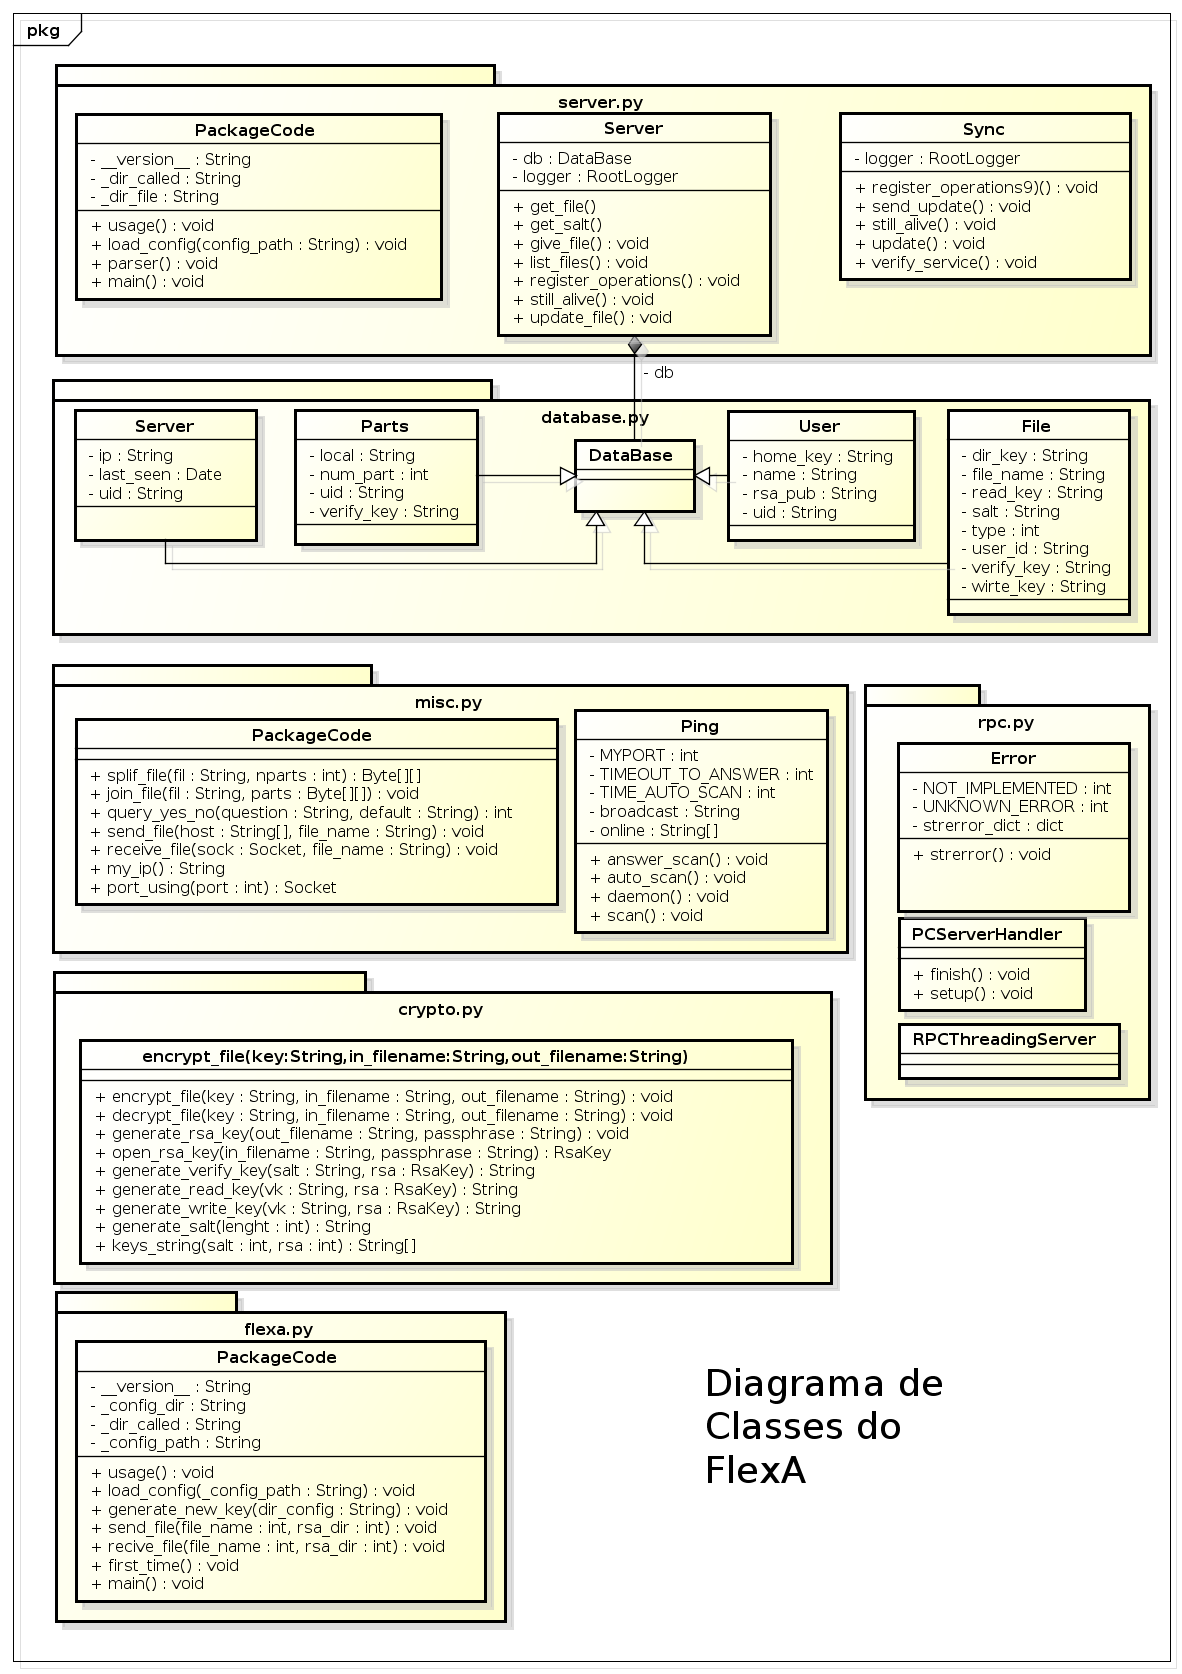
\includegraphics[width=12cm]{classesMario.png}
        \caption{Classes e pacotes (arquivos) que estruturam a versão atual do FlexA}
        \label{fig:classesMario}
        \end{figure}
             
        
        Para que o FlexA seja mais aberto e flexível é necessário realizar adaptações no código afim de fazer uma melhor separação das funções e dos módulos.
        
        \subsection{Diagrama de Casos de Uso}
        
        Para que fosse possivel elaborar a adaptação do projeto, num primeiro momento foi feito o levantamento dos requisitos do FlexA, junto com os objetivos de melhoria do código existente. Dessa forma foi elaborado um diagrama UML de casos de uso de acordo com ~\cite{umlCasosDeUso}. O diagrama com os casos de uso é apresentado na Figura \ref{fig:casosDeUsoGabriel}.
        
        \begin{figure}[!ht]
        \centering
        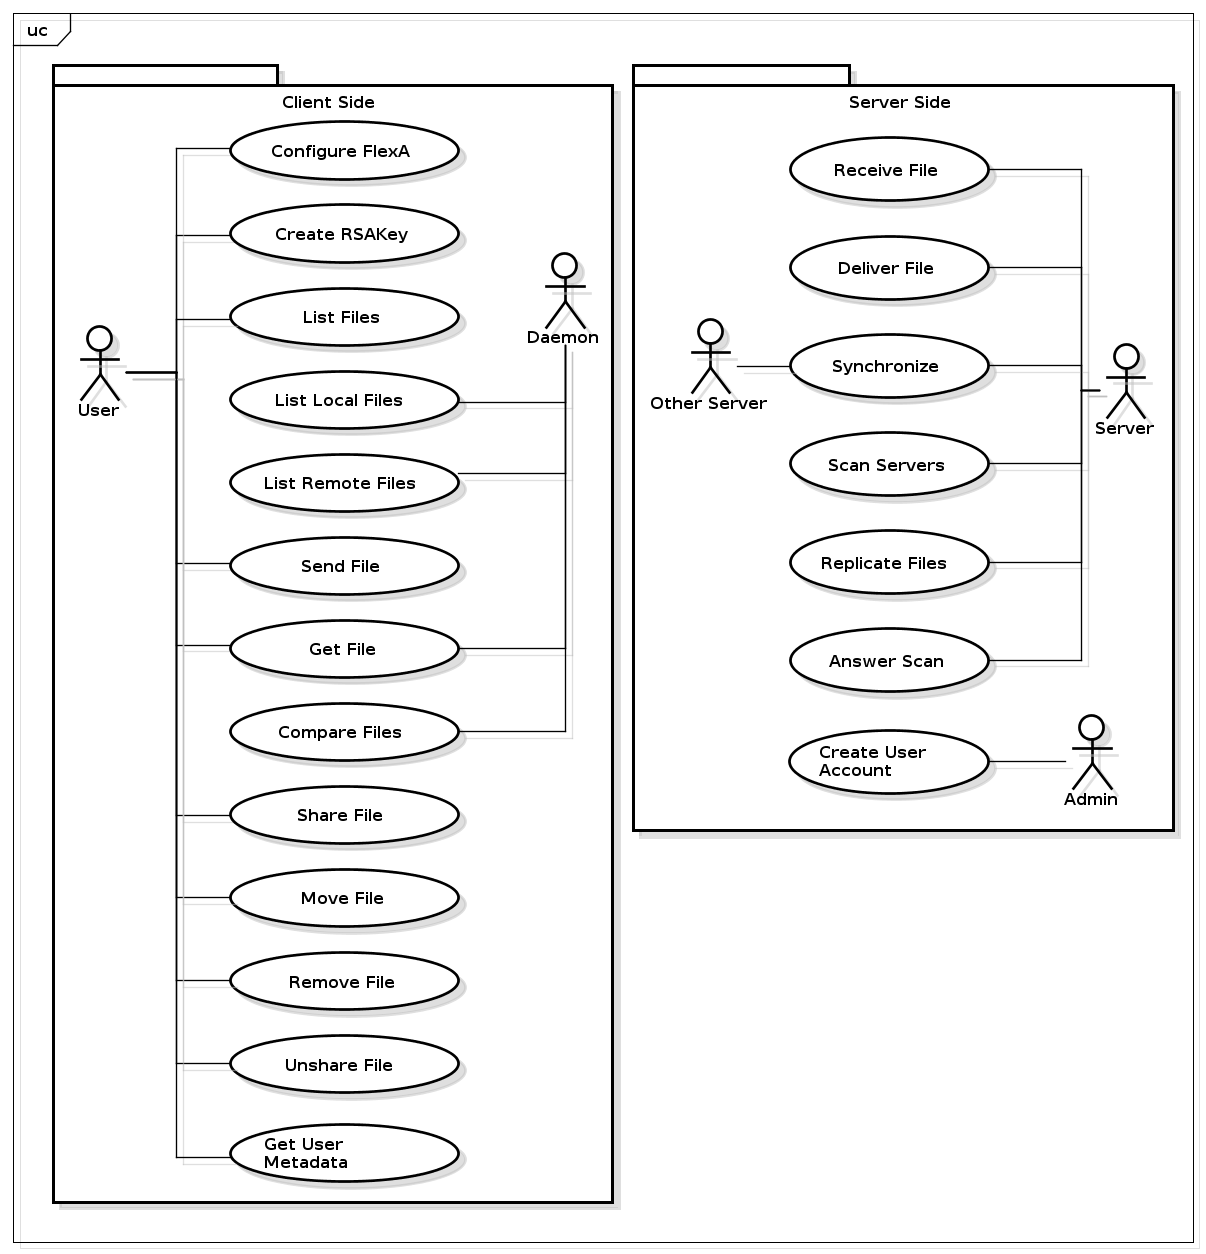
\includegraphics[width=12cm]{casosDeUsoGabriel.png}
        \caption{Diagrama de Casos de uso com os requisitos funcionais do FlexA.}
        \label{fig:casosDeUsoGabriel}
        \end{figure}
    
        Dos casos de uso apresentados na figura \ref{fig:casosDeUsoGabriel}, serão implementados e utilizados nesse trabalho apenas os referentes ao módulo cliente devido ao escopo do projeto. Os restantes foram definidos juntos para preparar os trabalhos futuros.
        
        \subsection{Interface de Comunicação Cliente-Servidor}
        
        Já com os objetivos do trabalho definidos, e uma documentação do que existia que permitisse entender o projeto, foi então formulada a interface que servirá de alicerce desse trabalho que será responsável por padronizar e fornecer as comunicações entre o cliente e o servidor. Essa interface, que é apresentada na figura   \ref{fig:interfaceComunicacao}, foi desenvolvida em reunião com os outros desenvolvedores do FlexA para que fossem atendidas todas as necessidades do trabalho atual e também do FlexA como um todo no futuro.
       
        \begin{figure}
        \centering
        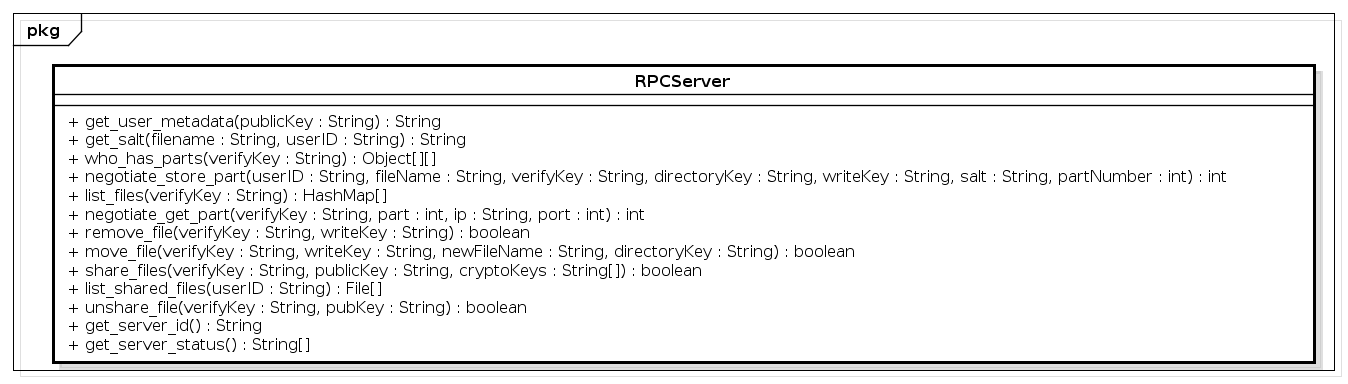
\includegraphics[width=15cm]{interfaceCom.png}
        \caption{Interface de comunicação dos servidores do FlexA.}
        \label{fig:interfaceComunicacao}
        \end{figure}
        
        Essa interface é de grande importância para o projeto, pois é ela que servirá como referência para o desenvolvimento do módulo cliente e também do módulo servidor, uma vez que define os métodos que deverão ser invocados durante a comunicação entre os clientes e os servidores, utilizando XML-RPC e independendo da linguagem utilizada.
        
        \subsection{Protocolos de Comunicação Cliente-Servidor}
        
        Com as funcionalidades que são esperadas do sistema e a interface de comunicação definida, foi feita a análise das comunicações entre cliente e servidor. Formalizou-se então os protocolos de comunicação, utilizando a notação para protocolos de comunicação apresentada em ~\cite{ross} que é mostrada na tabela \ref{tab:notacao}. 
        
        \begin{table}[!ht]
        
        \centering
        \begin{tabular}{|l|l|}
        \hline
        
        $C$ & módulo cliente \\
        \hline
        $S$ & módulo servidor \\
        \hline
        $privKey_{X}$ & chave privada $X$ \\
        \hline
        $pubKey_{X}$ & chave pública $X$ correspondente a $privKey_{X}$\\
        \hline
        $C \rightarrow S : dado$ & $C$ envia $dado$ para $S$\\
        \hline
        $C \rightarrow S : {dado}_{pubKey_{x}}$ & $C$ envia $dado$ criptografado com a chave pública $X$ para $S$\\
        \hline

        \end{tabular}
        \caption{Notação utilizada para definição de protocolos de comunicação ~\cite{ross}.}
        \label{tab:notacao}
        \end{table}
        
        Formalizadas as definições que serão utilizadas a seguir, são apresentados os protocolos para as comunicações. Esses protocolos foram elaborados com base no código fonte ~\cite{mario} e na interface de comunicação apresentada, já inserindo as adaptações para fornecer maior modularização, compatibilidade e segurança ao sistema.
        
        \subsubsection{Protocolos de manipulação de arquivos}
        
        A primeira formalização é o protocolo para solicitação dos metadados do usuário, que é feita quando o FlexA é iniciado pela primeira vez ou caso seja necessário obter o \textit{userID} do usuário. Isso é feito com base em sua chave pública previamente cadastrada no sistema por um administrador. O protocolo é apresentado na figura \ref{fig:protMetadadosUsuario}. Esse protocolo é implementado pela função \textit{get\_user\_metadata}, que é apresentada na figura \ref{fig:interfaceComunicacao}.
        
        \begin{figure}[!ht]
        
        \bordaProtocolo{
                $C \rightarrow S: pubKey_{C}$ \\
                $S \rightarrow C: \{userID,homeKey\}_{pubKey_{C}}$
        }
        
        \caption{Protocolo de requisição dos metadados de um usuário com base na sua chave pública.}
        \label{fig:protMetadadosUsuario}
        \end{figure}
        
        Com os metadados do usuário (\textit{userID} e \textit{homeKey} que é o identificador de sua pasta raiz) o usuário pode começar a utilizar o sistema enviando e recebendo arquivos.
        
        Para que o usuário possa enviar um arquivo para o sistema é necessário verificar se existe um arquivo com o mesmo nome no mesmo endereço especificado através do \textit{salt}. Caso o arquivo não exista ainda, é feito o cadastro e solicitado o \textit{salt} referente ao arquivo. Na figura \ref{fig:protGetSalt} é formalizado o protocolo de requisição do \textit{salt} de um arquivo. É importante ressaltar que \textit{fileName} é composto pelo nome completo do arquivo com o diretório em que o arquivo se encontra. Esse endereço é relativo ao diretório mapeado do FlexA para o usuário. Esse protocolo é implementado pela função \textit{get\_salt}, que é apresentada na figura \ref{fig:interfaceComunicacao}.

        \begin{figure}[!ht]
        \bordaProtocolo{
            $C \rightarrow S: fileName,userID$ \\
            $S \rightarrow C: salt$
        }
        \caption{Requisição do \textit{salt} de um arquivo.}
        \label{fig:protGetSalt}
        \end{figure}
        
        Caso o \textit{salt} retornado pelo servidor seja igual $0$ é assumido que esse arquivo ainda não existe no servidor, e então o próprio cliente gera um \textit{salt} para esse arquivo.
        
        Já com o \textit{salt}, o módulo cliente gera o trio de chaves para o arquivo (VK, RK e WK) de acordo com a figura \ref{fig:chavesFlexa} , criptografa o arquivo utilizando a RK, faz a divisão do arquivo em $N$ porções de acordo com o tamanho do arquivo, ($N$ e o tamanho do arquivo são configurações definidas pelo usuário) caso necessário e envia cada porção para um servidor. Primeiro o módulo cliente faz o cadastro do arquivo no servidor e então envia as porções. Na figura \ref{fig:protSendFile} é descrito o protocolo utilizado no cadastro do arquivo, onde $N$ é o número de porções em que o arquivo foi dividido, $directoryKey$ é o identificador do diretório que o arquivo está e $fileType$ é o tipo do arquivo (diretório ou arquivo comum). Esse protocolo é implementado pela função \textit{negociate\_store\_part}, que é apresentada na figura \ref{fig:interfaceComunicacao}.
        
        \begin{figure}[!ht]
        \bordaProtocolo{
            Para $i$ de $1$ até $N$: \\
            $C \rightarrow S_{i}: userID,fileName,verifyKey,directoryKey,writeKey,salt,partNumber_{i}$ \\
            $S_{i} \rightarrow C: port $
        }
        
        \caption{Cadastro do arquivo nos servidores e negociação da porta de envio do arquivo}
        \label{fig:protSendFile}
        \end{figure}
        
        Após o cadastro do arquivo e a negociação da porta de transmissão do arquivo, é feita a transmissão do arquivo em uma nova conexão com o servidor na porta $port$.
        
        Com a negociação pronta basta enviar para o servidor a porção correspondente. Essa comunicação é definida conforme o protocolo mostrado na figura \ref{fig:protSendFileData}. Esse protocolo é implementado através de \emph{sockets}, sem o uso do XML-RPC, por questões de desempenho.
        
        \begin{figure}[!ht]
        \bordaProtocolo{
            Para $i$ de $1$ até $N$: \\
            $C \rightarrow S_{i}: filePart_{i}$
        }
        \caption{Transmissão das porções dos arquivos aos servidores, feito via socket.}
        \label{fig:protSendFileData}
        \end{figure}
        
        
        Com os protocolos já definidos é possível enviar um arquivo para o servidor. Mas ainda não é possível recuperá-lo. A seguir serão tratados os protocolos envolvidos na recuperação dos arquivos enviados aos servidores.
        
        Para recuperar um arquivo, é de grande importância a capacidade de listar os arquivos de um diretório. Para essa ação é utilizado o protocolo da figura \ref{fig:protListFiles}. Esse protocolo é implementado pela função \textit{list\_files}, que é apresentada na figura \ref{fig:interfaceComunicacao}.
        
        \begin{figure}[!ht]
        \bordaProtocolo{
            $C \rightarrow S: directoryKey$\\
            $S \rightarrow C: metaFile_{0}, metaFile_{1}, metaFile_{2},...,metaFile_{n}$
        }
        \caption{Requisição da lista dos arquivos em um diretório}
        \label{fig:protListFiles}
        \end{figure}
        
        Ao requisitar ao servidor os arquivos do diretório referenciado por $directoryKey$, o servidor manda pacotes de informação $metaFile$ referente aos arquivos. Cada pacote desse é composto por:
        \begin{itemize}
            \item nome do arquivo
            \item tamanho do arquivo
            \item dono do arquivo
            \item data de criação
            \item data de modificação
        \end{itemize}
        
        Essas características do arquivo são enviadas junto com o nome do arquivo para evitar acessos desnecessários ao servidor para recuperar cada uma dessas informações posteriormente. Isso influencia no tempo de resposta do sistema.
        
        Com a lista dos arquivos, o usuário pode requisitar um arquivo específico ao servidor. Ao requisitar o arquivo, o módulo cliente faz a solicitação do \textit{salt} referente ao arquivo pelo atributo nome, com essa informação gera o trio de chaves do arquivo. Com o identificador do arquivo (\textit{verify key}), o cliente solicita a um servidor uma lista com quais servidores possuem as porções do arquivo. Essa comunicação é formalizada na figura \ref{fig:protWhoHasParts}. Esse protocolo é implementado pela função \textit{who\_has\_parts}, que é apresentada na figura \ref{fig:interfaceComunicacao}.
        
         \begin{figure}[!ht]
        \bordaProtocolo{
            $C \rightarrow S: VK, userID$ \\
            $S \rightarrow C: (S_{0},1),(S_{0},2),(S_{1},1),(S_{1},3),(S_{2},2),(S_{2},3),...$
        }

        \caption{Já com a \textit{verify key}, é solicitado uma lista dos servidores que possuem as partes do arquivo}
        \label{fig:protWhoHasParts}
        \end{figure}
        
        Ao fazer a solicitação de quais servidores possuem as partes do arquivo desejado, o cliente recebe uma lista de registros de quais servidores possuem qual parte do arquivo, no seguinte formato: ($SERVIDOR$,$PARTE DO ARQUIVO$). Esse é o formato utilizado na figura \ref{fig:protWhoHasParts}.
        
        Com a lista dos servidores que possuem as partes do seu arquivo o cliente pode finalmente requisitar as partes do arquivo. Esse processo é feito de acordo com o protocolo apresentado pela figura \ref{fig:protNegociateGetPart} e é implementado pela função \textit{negociate\_get\_parts}, que é apresentada na figura \ref{fig:interfaceComunicacao}.
        
        \begin{figure}[!ht]
        \bordaProtocolo{
            Para $i$ de $1$ até $N$:\\
                $C \rightarrow S_{i}: verifyKey,part{i},ip,port$
        }
        \caption{Módulo cliente envia informação para os servidores, negociando o recebimento das partes}
        \label{fig:protNegociateGetPart}
        \end{figure}
        
        Esse protocolo diz que o cliente é quem irá abrir a conexão para receber o arquivo, e o servidor ira se conectar com o cliente utilizando o $ip$ e $port$ para isso. Após conectado com o cliente o servidor enviará o arquivo para o cliente baseado pelo protocolo apresentado pela figura\ref{fig:protGetPart}. Uma vez que esse protocolo também não é feito via XML-RPC não é definida uma função específica.
        
        \begin{figure}[!ht]
        \bordaProtocolo{
            Para $i$ de $1$ até $N$:\\
                $S_{i} \rightarrow C: filePart_{i}$
        }
        \caption{Servidores enviando porções do arquivo para o cliente}
        \label{fig:protGetPart}
        \end{figure}
        
        
        
        Uma vez que o cliente tenha todas as partes do arquivo a junção dessas partes é feita e o arquivo é descriptografado utilizando a chave de criptografia \textit{read key} que apenas o cliente possui.
        
        A operação de atualização de um arquivo nos servidores é equivalente a remover o arquivo atual e cadastrar um novo arquivo. Como o protocolo de envio de arquivos já foi apresentado nas figuras \ref{fig:protSendFile} e \ref{fig:protSendFileData}, são feitas a seguir a definição do protocolo de remoção de um arquivo dos servidores. Esse protocolo é apresentado na figura \ref{fig:protRemoveFile} e é implementado pela função \textit{remove\_file} da figura \ref{fig:interfaceComunicacao}.
        
        \begin{figure}[!ht]
        \bordaProtocolo{
            Para $i$ de $1$ até $N$:
            $C \rightarrow S_{i}: verifyKey,writeKey$
        }
        \caption{Protocolo que define a remoção das partes de um arquivo.}
        \label{fig:protRemoveFile}
        \end{figure}
        
        
        Como definido pelo protocolo de remoção de arquivos, o cliente deve fazer a busca dos servidores que possuem as partes do arquivo desejado, utilizando o protocolo já especificado na figura \ref{fig:protWhoHasParts}. Então o cliente envia ao servidor o identificador do arquivo que deseja excluir e a chave de escrita no arquivo. O cliente deve fazer isso para todos os servidores. Essa operação é feita no cliente para manter a filosofia do FlexA de trazer a complexidade de processamento e comunicação para o cliente.
        
        Além de enviar, listar, excluir e atualizar os arquivos remotos, uma operação que também é de grande importância é a de mover arquivos para outro diretório. No FlexA essa operação é feita totalmente no módulo servidor de forma que o cliente não necessita enviar novamente o arquivo ao move-lo de diretório. Essa operação tem o protocolo de comunicação especificado na figura \ref{fig:protMoveFile}, e é implementado pela função \textit{move\_file} da figura \ref{fig:interfaceComunicacao}.
        
        \begin{figure}[!ht]
        \bordaProtocolo{
            $ C \rightarrow S: verifyKey,writeKey,destinationFileName, directoryKey $
        }
        \caption{Protocolo para mover um arquivo.}
        \label{fig:protMoveFile}
        \end{figure}
        
        
        Outro recurso muito importante do FlexA é o compartilhamento de arquivos, que é implementado através do compartilhamento das chaves de criptografia. Para que seja possível fazer o compartilhamento e armazenar o estado deles o servidor cadastra esses dados criptografados, utilizando a chave pública do usuário que recebe a autorização para acessar o arquivo compartilhado. O protocolo de comunicação para a execução desse procedimento é apresentado na figura \ref{fig:protShareFile}, e é implementado pela função \textit{share\_file} da figura \ref{fig:interfaceComunicacao}.
        
        \begin{figure}[!ht]
        \bordaProtocolo{
            $C \rightarrow S: verifyKey, pubKey_{B}, \{accessKeys\}_{pubKey_{B}}$
        }
        \caption{Protocolo para o compartilhamento de arquivos}
        \label{fig:protShareFile}
        \end{figure}
        
        Como mostrado na figura \ref{fig:protShareFile}, o cliente envia as chaves de acesso que desejar ao usuário $B$, cifrando-as com a chave pública de $B$.
        
        
        Para que seja possível executar o procedimento de compartilhamento de arquivos é necessário obter a chave pública de um usuário. Esse procedimento é feito através do compartilhamento da chave pública entre os próprios usuários, sem o uso do sistema para isso.
        
        Quando o usuário B desejar requisitar o arquivo que foi compartilhado com ele, o mesmo protocolo de recebimento de arquivos é utilizado, apenas omitindo a parte de solicitação do \textit{salt}, pois já possui as chaves de acesso ao arquivo. Para saber quais arquivos o usuário $B$ tem acesso ele deve listar os arquivos compartilhados cadastrados com sua chave pública, utilizando o protocolo exibido na figura \ref{fig:protListSharedFiles}, que é implementado pela função \textit{list\_shared\_files} da figura \ref{fig:interfaceComunicacao}.
        
        
     \begin{figure}[!ht]
        \bordaProtocolo{
        $C \rightarrow S: userID$
        }
        \caption{Protocolo para o listar os arquivos compartilhados com um usuário.}
        \label{fig:protListSharedFiles}
        \end{figure}
        
        Por fim, após compartilhar um arquivo, caso seja necessário remover o compartilhamento, é necessário refazer a criptografia do arquivo, removê-lo do sistema e cadastrá-lo novamente, já que as chaves de acesso foram fornecidas a outro usuário no compartilhamento. Para remover o acesso a um arquivo compartilhado é utilizado o protocolo apresentado na figura \ref{fig:protRemoveShare} que é implementado pela função \textit{unshare\_file} da figura \ref{fig:interfaceComunicacao}.
        
        \begin{figure}[!ht]
        \bordaProtocolo{
            $C \rightarrow S: verifyKey,pubKey_{B}$
        }
        \caption{Remove o acesso do usuário $B$ a um arquivo compartilhado pelo usuário $C$}
        \label{fig:protRemoveShare}
        \end{figure}
        
        Vale ressaltar que embora seja custoso computacionalmente ter que recriptografar os arquivos que foram compartilhados, o FlexA possui bons mecanismos para fazer essa operação, que foram propostos ~\cite{silas}, estudados e implementados por ~\cite{leandro} 
        
        
        Esses são todos os protocolos que coordenam a comunicação entre o módulo cliente e o servidor (e vice e versa) para a manipulação de arquivos. Além desses protocolos ainda existem os que são utilizados para a obtenção dos metadados dos servidores, que são apresentados a seguir.
        
        
        \subsubsection{Protocolos de obtenção de metadados dos servidores}
        
        Para que o cliente possa se comunicar com um servidor ele deve conhece-lo, isso inclui saber seu \textit{serverID}, e o estado atual dos recursos do servidor.
        
        O protocolo que rege a comunicação para a obtenção do ID do servidor é apresentado na figura \ref{fig:protGetServerID} e é implementado pela função \textit{get\_server\_id} da figura \ref{fig:interfaceComunicacao}.

        \begin{figure}[!ht]
        \bordaProtocolo{
            $S \rightarrow C: serverID$
        }
        \caption{Servidor envia seu \textit{serverID} para cliente.}
        \label{fig:protGetServerID}
        \end{figure}
    
        Além do \textit{serverID} é importante que o servidor tenha um meio de passar informações sobre o estado atual de seus recursos para o cliente. Esse protocolo é de grande importância, pois permite que futuramente possam ser incorporados  os mecanismos de balanceamento de carga propostos e implementados por ~\cite{danilo}.
        O protocolo para a obtenção do estado do servidor é apresentado na figura \ref{fig:protServerGetStatus} e é implementado pela função \textit{get\_server\_status} da figura \ref{fig:interfaceComunicacao}.
        
         \begin{figure}[!ht]
         \bordaProtocolo{
            $S \rightarrow C: status_{1}, status_{2}, status_{3}, ..., status_{n} $
         }
         \caption{Servidor envia para cliente métricas sobre seu estado atual.}
         \label{fig:protServerGetStatus}
         \end{figure}
        
        Com todos esses protocolos definidos e formalizados o sistema possui documentação suficiente para passar para a faze de implementação da versão Android do módulo cliente.
        
        \section{Adaptação do servidor em Python}
        
        % Implementação das funções da interface de comunicação
        % alterações no banco de dados (share)
        
        Com relação ao módulo servidor, a parte envolvida nesse trabalho é a de comunicação com o cliente. Dessa forma foi necessário implementar as funções definidas na figura \ref{fig:interfaceComunicacao}, utilizando os protocolos definidos na seção anterior.
        
        As novas funções foram agregadas ao servidor, de forma que ele ainda mantenha a compatibilidade com o módulo cliente em Python existente. Quando o módulo cliente for remodelado para trabalhar igual ao novo cliente desenvolvido, será necessário apenas remover as funções de comunicação antigas e sem uso do servidor.
        
        Outra alteração que se fez necessária no módulo servidor foi a criação de uma nova entidade para armazenar os metadados do compartilhamento dos arquivos entre os usuários. Isso foi feito com a criação de uma nova classe para o mapeamento objeto-relacional utilizado ou \textit{Object-Relational Mapping} (ORM) com SQLAlchemy e SQLite. Essa nova classe é apresentada na figura \ref{fig:shareORM}. Essas alterações foram feitas de acordo com o que é recomendado por ~\cite{sqlalchemy}.
        
        \begin{figure}
        \centering
        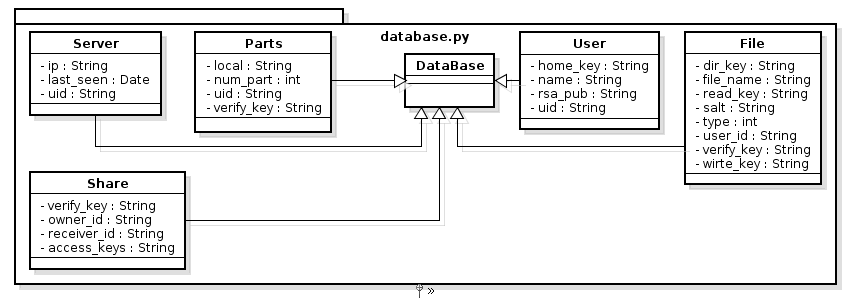
\includegraphics[width=14cm]{shareORM.png}
        \caption{Diagrama de classes mostrando a classe \textit{Share}, responsável por armazenar os metadados sobre o compartilhamento dos arquivos.}
        \label{fig:shareORM}
        \end{figure}
        
        \section{Módulo Cliente para Android}
        
        % - Estudo do Android
        % - Organização do projeto
        % - Modularização
        % - GUI
     
        Um módulo cliente implementado em outra arquitetura é de grande interesse como caso de teste de que as alterações propostas tornam o FlexA capaz de executar em sistemas diferentes e também testar sua nova interface de comunicação, e ainda fornecer ao usuário outra alternativa de uso do sistema.
        
        \subsection{Organização}
        
        Uma das principais contribuições do cliente para Android ao projeto original é a modularização e organização do projeto, separando as funcionalidades e implementação de recursos em pacotes bem definidos com o uso de interfaces de desenvolvimento que forneçam flexibilidade ao projeto.
        
        A modularização do trabalho desenvolvido é mostrada através da arvore de pacotes. Dentro de cada pacote permanecem apenas implementações de tarefas do mesmo tipo. Essa arvore é apresentada na figura \ref{fig:arvorePacotesAndroid}.
        
        \begin{figure}[!ht]
        \centering
        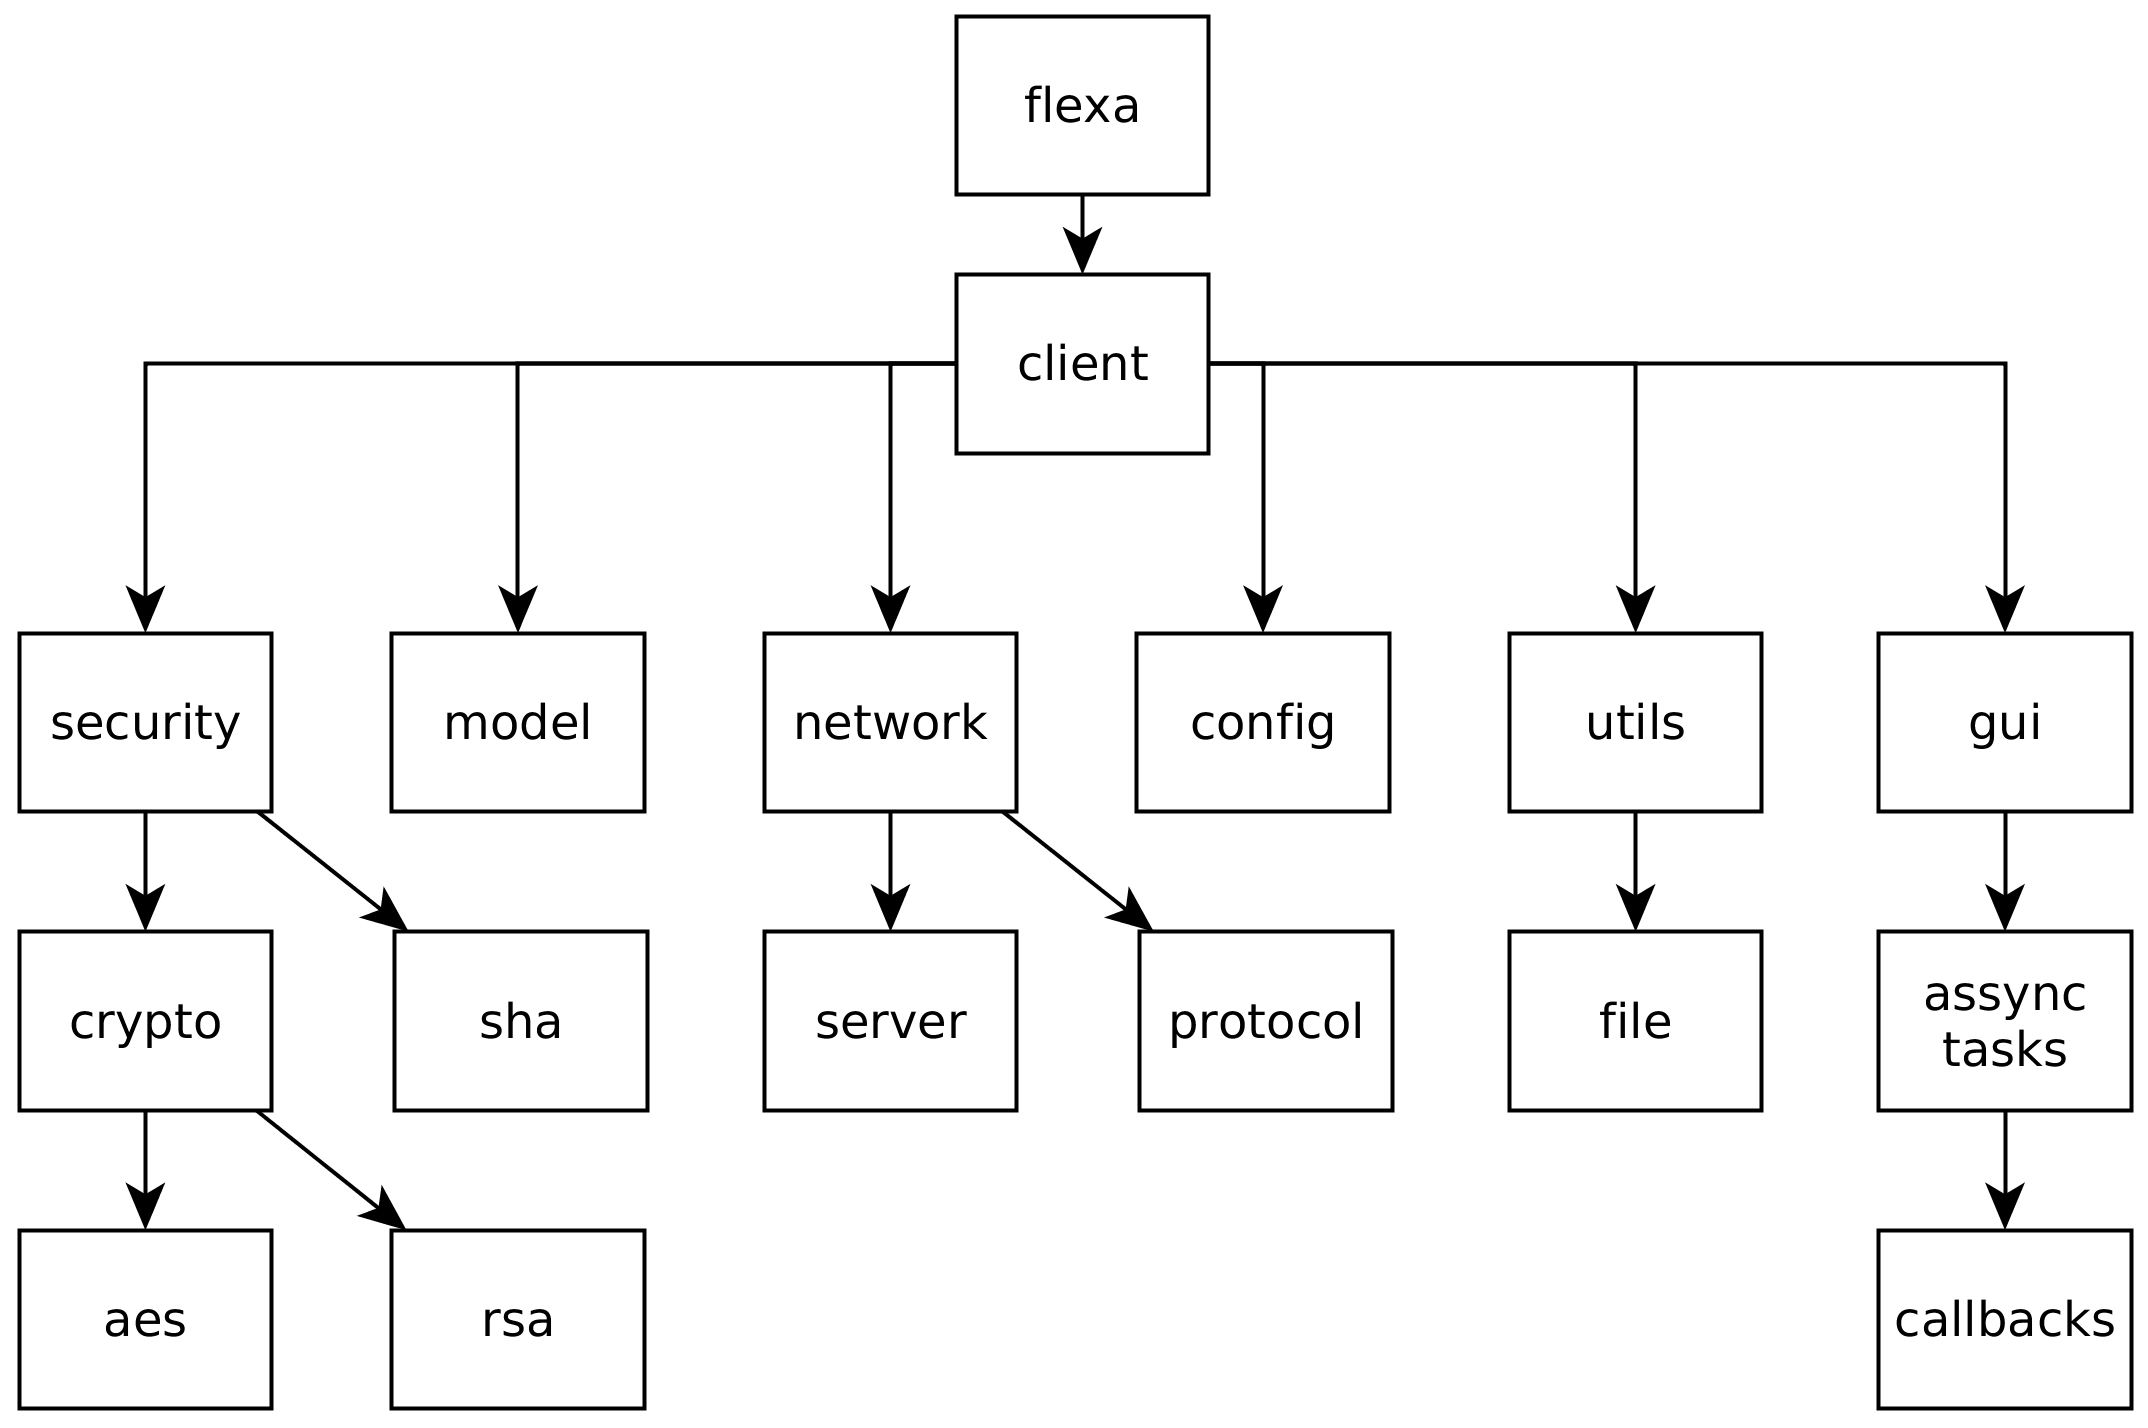
\includegraphics[width=14cm]{pacotesGabriel.png}
        \caption{Hierarquia de pacotes que compõe o módulo Cliente para Android}
        \label{fig:arvorePacotesAndroid}
        \end{figure}
        
        Da forma como o sistema está estruturado, quando no futuro for necessário alterar o módulo cliente ou até mesmo implementar o módulo servidor para Android ou em Java, essa tarefa será bem simples de ser feita pois toda a estrutura do sistema estará pronta, e assim o módulo servidor poderá importar apenas os pacotes que necessita, sem que para isso, seja necessário carregar junto funções e bibliotecas desnecessárias.
        
        \subsection{Modularização e Flexibilidade}
        
        A modularização do projeto ocorre não apenas pelo uso de pacotes e separação do código em classes bem definidas. Para que o projeto possa se manter a longo prazo flexível, são utilizadas diversas interfaces para garantir que caso seja necessário realizar alterações em mecanismos de comunicação e na interface gráfica do usuário ou \textit{Graphical User Interface} (GUI), essas alterações sejam simples de serem implementadas. Os principais pontos são listados a seguir.
        
         \subsubsection{Encapsulamento da complexidade do FlexA}
         
        Embora o XML-RPC forneça um alto grau de encapsulamento da comunicação, ainda é necessário obter uma forma de simplificar o acesso as funções fornecidas pelos servidores XML-RPC e toda a sequência ações que devem ser feitas. Esse encapsulamento é obtido utilizando a classe \textit{Client}, que é mostrada na figura \ref{fig:clientClass}. Dessa forma, caso aconteça qualquer alteração nos protocolos ou nos parâmetros o resto do cliente não precisa ser alterado, ou irá precisar de apenas pequenos ajustes.
        
        \begin{figure}[!ht]
        \centering
        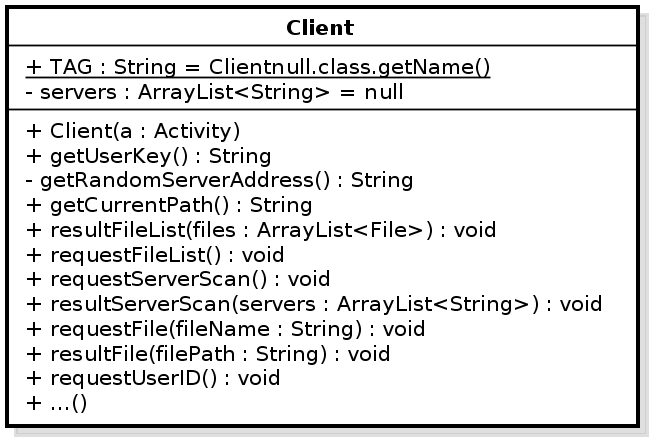
\includegraphics[width=14cm]{classeCliente.png}
        \caption{Classe \textit{Client}, responsável por ocultars servidores e manipulação dos arquivos.}
        \label{fig:clientClass}
        \end{figure}
        
        
         \subsubsection{Encapsulamento da comunicação com os servidores que utilizam XML-RPC}
         
        Ainda sim, para isolar o módulo cliente do cliente XML-RPC utilizado existe a classe \textit{FlexaServer} que é apresentada na figura \ref{fig:flexaServer}. Essa classe é a responsável por se conectar com os servidores RPC e implementar as operações  do lado do cliente mostradas na seção anterior na figura \ref{fig:interfaceComunicacao}.
        
        \begin{figure}[!ht]
        \centering
        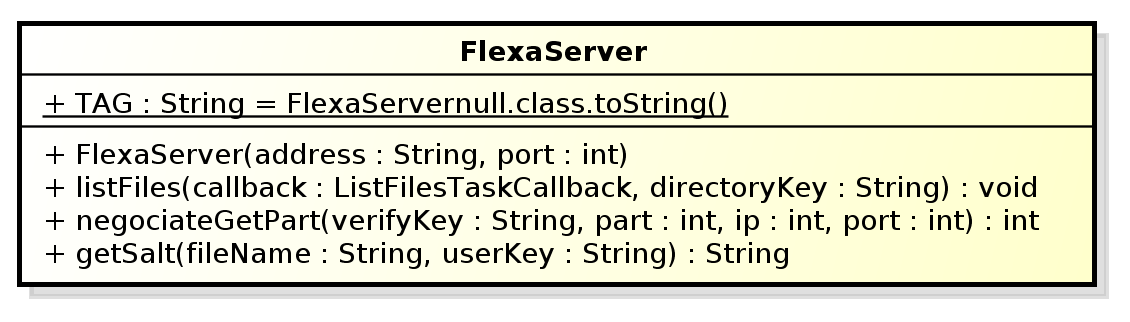
\includegraphics[width=14cm]{flexaServerClass.png}
        \caption{Interface de comunicação com os servidores XML-RPC.}
        \label{fig:flexaServer}
        \end{figure}
        
        
        \subsection{Interface Gráfica do Usuário no Android}
        
        Com as classes \textit{FlexaServer} e \textit{Client}, o resto do módulo cliente fica encapsulado e livre da comunicação com os servidores, devendo assim apenas cuidar da entrada e saída dos dados e da comunicação com o usuário do sistema através de uma interface gráfica. Uma das telas do sistema é exibida na figura \ref{fig:flexaGuiModel}.
        
        \begin{figure}[!ht]
        \centering
        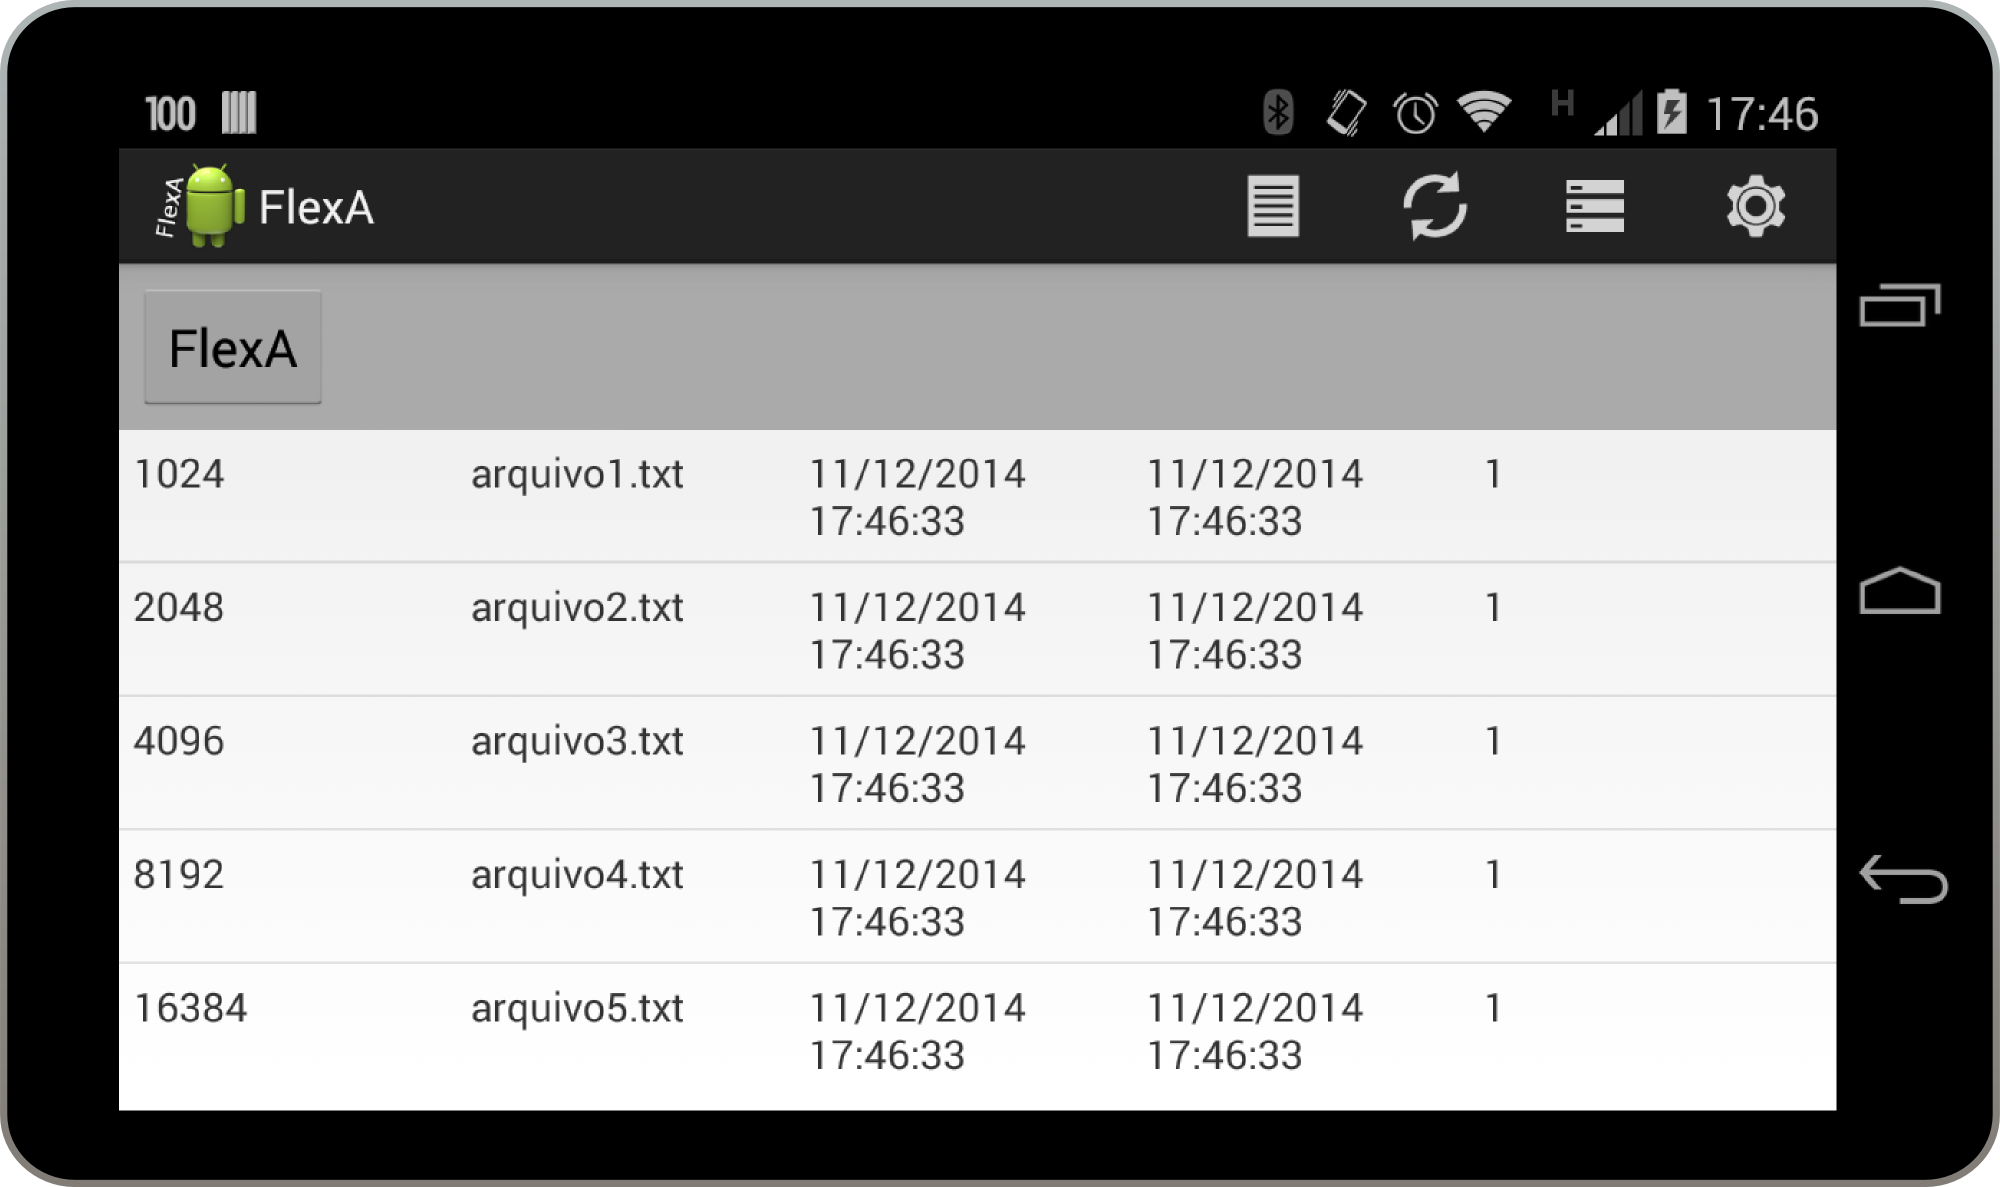
\includegraphics[width=14cm]{flexaGuiModel.png}
        \caption{Exemplo de interface gráfica listando os arquivos do usuário.}
        \label{fig:flexaGuiModel}
        \end{figure}
        
        A utilização de uma GUI para Android, embora seja necessária para a comodidade do usuário final, é bem mais complexa que a implementação para interface de linha de comando ou \textit{Command-line Interface} (CLI) que existe atualmente no cliente em Python. Para obter um resultado satisfatório no uso de uma GUI, é necessário tratar de forma assíncrona e também utilizar \textit{callbacks} nas operações de entrada e saída, de modo a evitar o congelamento do aplicativo ao realizar essas tarefas ~\cite{androidAssyncTask}. Dois exemplos dessas tarefas são mostradas na figura \ref{fig:assyncCallback}.
        
        \begin{figure}[!ht]
        \centering
        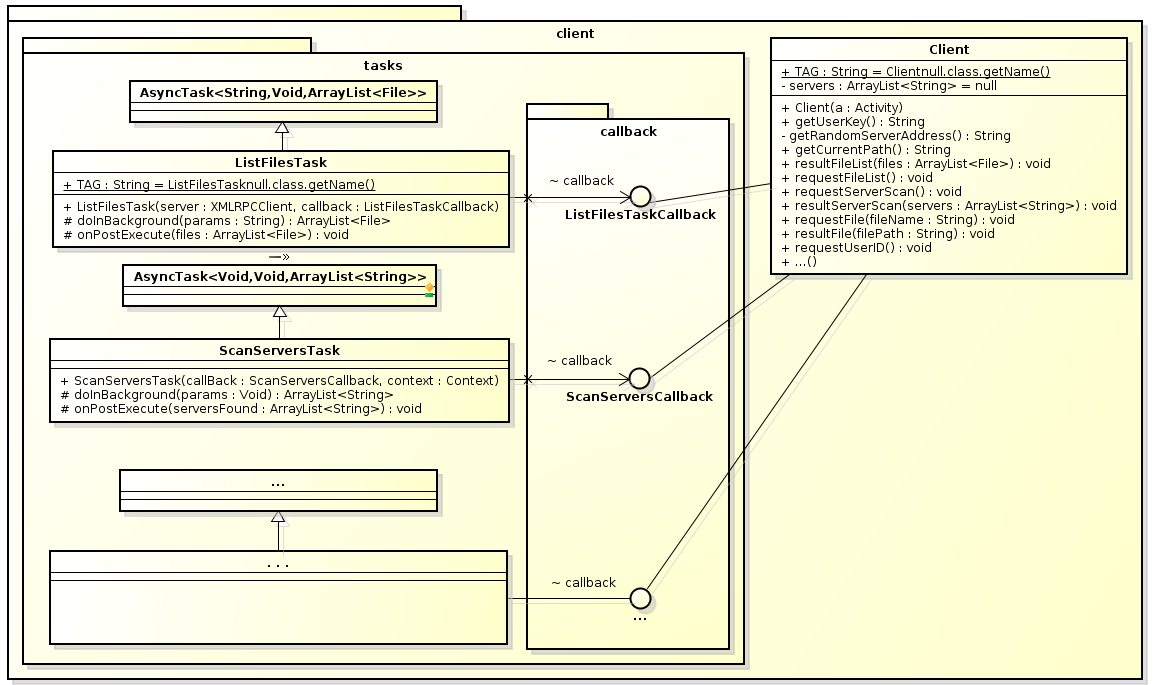
\includegraphics[width=14cm]{assyncCallback.png}
        \caption{Exemplo de duas tarefas assíncronas, uma feita via XML-RPC (\textit{listFiles}) e outra via \textit{socket} (\textit{scanServers}).}
        \label{fig:assyncCallback}
        \end{figure}
        
    Junto com as tarefas assíncronas estão também como exemplo uma parte da classe \textit{Splash} e da interface \textit{FlexaGui} que fazem a conexão com a interface gráfica do cliente que estão destacadas com a cor cinza claro.
    
    Na figura \ref{fig:classesSeg} são apresentados detalhes das classes responsáveis por realizar o processo de segurança com os mecanismos de \textit{hash} e criptografia. Ainda nesta figura estão as classes que fornecem o acesso aos arquivos para a divisão das porções.
    
        \begin{figure}[!ht]
        \centering
        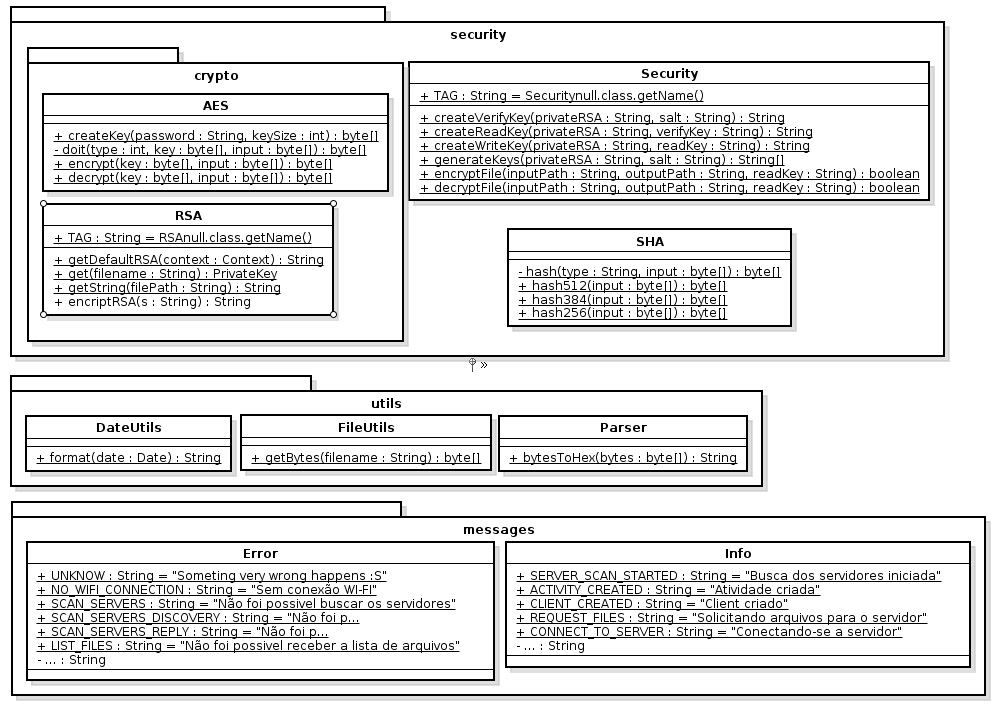
\includegraphics[width=14cm]{classesSegurancaUtils.png}
        \caption{Seções das classes de criptografia e acesso a arquivos.}
        \label{fig:classesSeg}
        \end{figure}
        
    Por fim estão as telas desenvolvidas que fornecem ao usuário acesso as configurações do FlexA, facilitando bastante o processo que anteriormente era feito realizando edições manuais no código fonte. Essas telas são apresentadas na figura \ref{fig:config}.
    
        \begin{figure}[!ht]
        \centering
        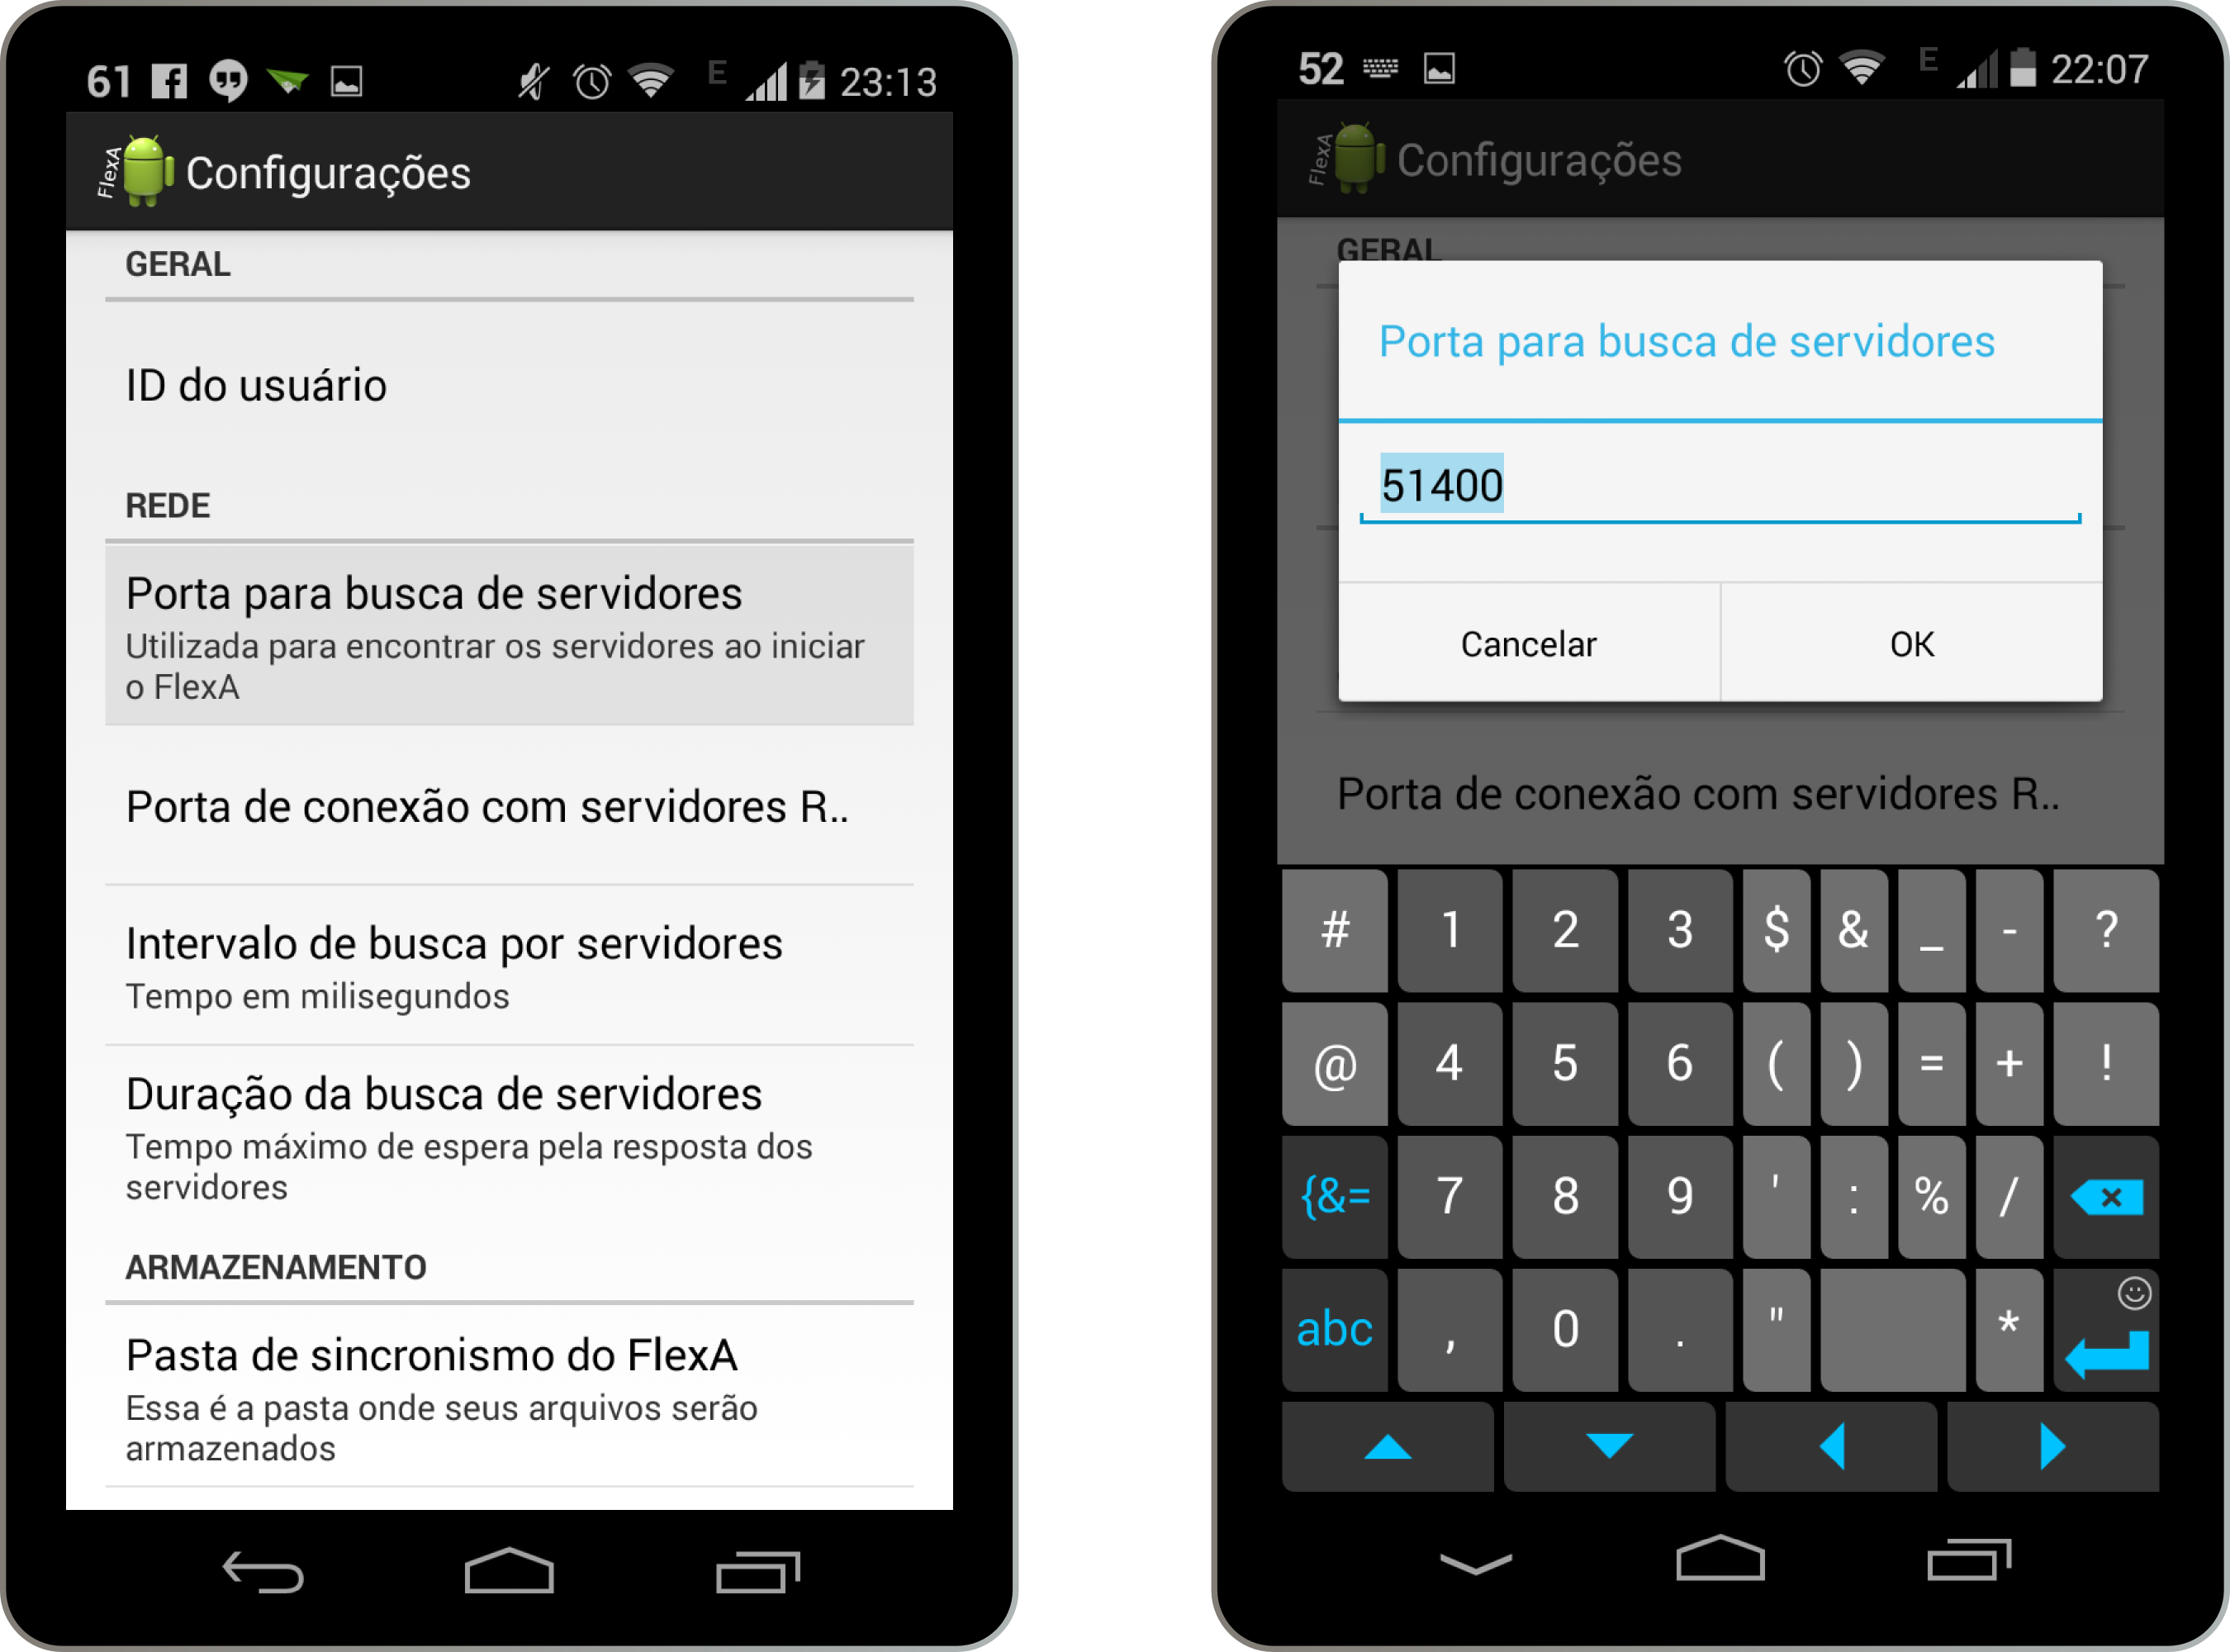
\includegraphics[width=14cm]{androidConfiguracoes.png}
        \caption{Módulo de configurações, fornece uma melhor usabilidade do sistema.}
        \label{fig:config}
        \end{figure}
        
    
    
%% Revisado por Gabriel Saraiva

\chapter{Testes e resultados}
\label{cap4}

Nesse capítulo serão apresentados os ambientes de testes e os resultados obtidos.

\section{Ambiente de Testes}

    O ambiente de testes utilizou os equipamentos disponíveis no laboratório do GSPD e um celular próprio.
    
    Esses equipamentos são:
    
    \begin{itemize}
    
    
    
    \item \textit{Cluster} heterogêneo com 16 nós:
    
    
        %
        %
        % - - - PEGAR PROCESSO DA FAPESP DO CLUSTER E INSERIR AQUI!!!
        % - - - COMO TEXTO! :)
        %
        %
        
        
    
        \begin{itemize}
        \item 8 nós equipados Intel(R) Core(TM) i7, 16GB de RAM, HD de 500GB
        \item 8 nós com Intel(R) Pentium(R) Dual, 4 GB de RAM, HD de 80GB
        \item Conexão 10/100/1000
        \end{itemize}
        
    \item \textit{Tablet} Samsung GALAXY Note 10.1 - 2014 (referente ao processo FAPESP 2012/02926-5):
        
        \begin{itemize}
            \item Android 4.3 (Jelly Bean)
            \item 3 GB de memória RAM
            \item 16GB de armazenamento interno (\textit{flash})
            \item bateria de 8220 mAh
            \item Chipset Qualcomm Snapdragon 800
            \item CPU Quad-core 1.9 GHz Cortex-A15
            \item GPU Adreno 330
        \end{itemize}
        
    \item \textit{Smart-phone} Motorola Moto X XT1058:
    
        \begin{itemize}
            \item Android  4.4.4 (KitKat)
            \item 2GB de memória RAM
            \item 16GB de armazenamento interno (\textit{flash})
            \item bateria de 2200 mAh
            \item Chipset Qualcomm MSM8960DT Snapdragon S4 Pro
            \item CPU Dual-core 1.7 GHz Krait 300
            \item GPU Adreno 320
            
        \end{itemize}
        
    \item Roteador Wi-fi Asus 300 Mbps
    
    \end{itemize}
    
     Os arquivos utilizados para realizar os testes são fotografias de altíssima resolução obtidas em  ~\cite{hubble}. Sendo uma fotografia de 6.6MB, outra de 15M e a maior de 172MB.
     
     
     Nos testes de desempenho e eficiência, para amenizar influências de outros processos e do sistema operacional, os testes foram realizados 10 vezes com intervalos aleatórios de 1 a 2 minutos. Os tempos utilizados nos gráficos são as médias dessas execuções.

\section{Integridade dos Dados}

    Segundo ~\citeonline{coulouris}, um dos principais deveres de um sistema de arquivos distribuídos é manter a integridade de seus arquivos, foram feitos testes de integridade dos arquivos, para verificar se o processo de criptografia e transmissão dos arquivos não danificaram os arquivos. 
    
    Inicialmente era calculado o \textit{hash} MD5 dos arquivos, que então eram copiados via cabo de dados para os dispositivos móveis. Então, eram transferidos e recuperados do FlexA via \textit{Wi-fi} e, então, eram novamente copiados para um computador via cabo de dados. Depois era calculado o \textit{hash} MD5 dos arquivos para mostrar a integridade dos mesmos. Na figura \ref{fig:testesIntegridade} são mostrados os resultados.

    \begin{figure}[!ht]
    \centering
    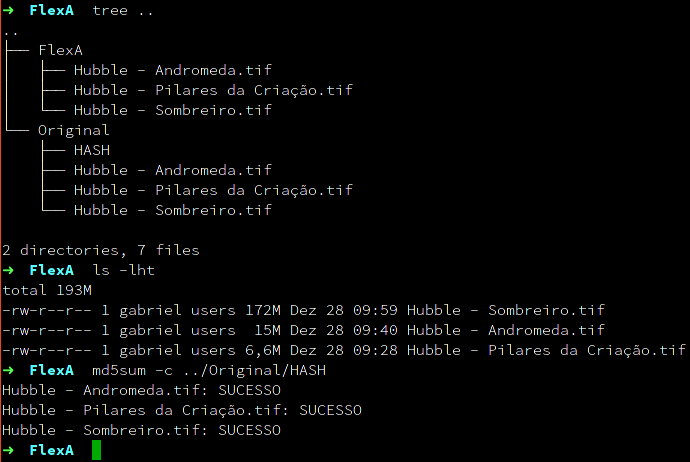
\includegraphics[width=14cm]{testeIntegridade.png}
    \caption{Teste de integridade dos arquivos com Android. Nenhum arquivo foi danificado durante os testes.}
    \label{fig:testesIntegridade}
    \end{figure}

    Todos os testes mostraram resultados positivos quanto a integridade dos arquivos ao serem enviados e retornarem pelo FlexA utilizando o Android.
    
\section{Compatibilidade do sistema}

    Como o módulo cliente implementado do FlexA deve ser compatível com o módulo existente, foram feitos testes semelhantes aos de integridade mostrado anteriormente, exceto que os arquivos eram inseridos no FlexA pelo cliente em Python e depois recuperados pelo cliente Android. Na figura \ref{fig:testeCompatibilidade} são apresentados os resultados desse teste.
    
    \begin{figure}[!ht]
    \centering
    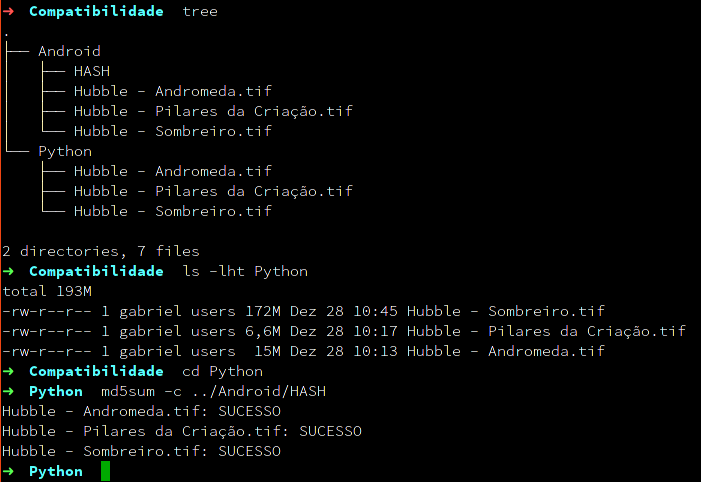
\includegraphics[width=14cm]{testeCompatibilidade.png}
    \caption{Teste de compatibilidade entre os dois módulos clientes do FlexA. Nenhum arquivo foi danificado durante os testes mostrando que os sistemas estão compatíveis.}
    \label{fig:testeCompatibilidade}
    \end{figure}
    
\section{Desempenho de criptografia}

    Esse teste mostra o tempo necessário para criptografar arquivos os arquivos de testes em cada um dos dispositivos móveis e também em um nó do primeiro grupo do \textit{cluster} (computadores com processador Intel Core i7) para comparação. Os resultados são mostrados na figura \ref{fig:testesCriptografia}.
    
    \begin{figure}[!ht]
    \centering
    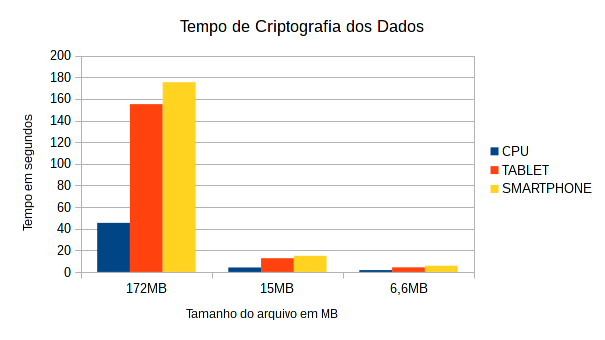
\includegraphics[width=14cm]{testeCriptografia.png}
    \caption{Teste de desempenho de criptografia com clientes diferentes do FlexA}
    \label{fig:testesCriptografia}
    \end{figure}
    
    Como esperado, o computador do \textit{cluster} foi capaz de criptografar os arquivos aproximadamente 3,4 vezes mais rápido que o \textit{tablet} e 3,8 vezes mais rápido que o \textit{smart-phone}.
    
\section{Desempenho de transmissão dos dados}

    Esse teste mostra o tempo necessário para transmitir os arquivos via Wi-fi para o FlexA. Os resultados são mostrados na figura \ref{fig:testeTransmissao}.
    
    \begin{figure}[!ht]
    \centering
    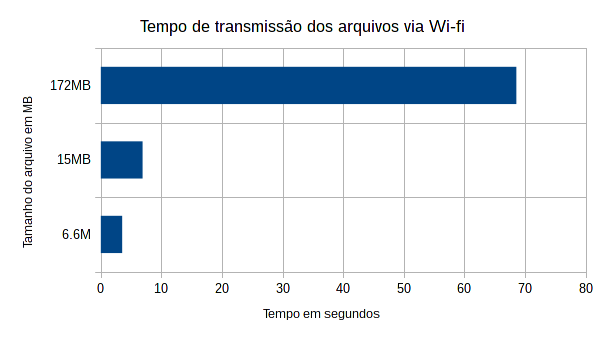
\includegraphics[width=14cm]{testeTransmissao.png}
    \caption{Teste de desempenho de transmissão de arquivos com clientes diferentes do FlexA}
    \label{fig:testeTransmissao}
    \end{figure}
    
    Como esperado, o particionamento do arquivo quase não influenciou na transmissão, uma vez que o gargalo nesse caso é a transmissão sem fio dos dados.
%% Revisado por Gabriel Saraiva

\chapter{Conclusão}
\label{cap5}

    A execução dese projeto mostrou-se muito benéfica ao FlexA como um todo, desde a formalização dos protocolos de comunicação, que tornou o sistema muito mais fácil de ser implementado e entendido, testado e no futuro expandido, até a implementação do cliente Android, que além de oferecer ao usuário outra alternativa mais simples para uso, ainda serviu para aprimorar a flexibilidade do projeto, ao torná-lo mais aberto e padronizado.
    
    Com os testes executados, foi possível perceber principalmente que o sistema está se comportando de forma esperada e que embora o FlexA não seja um sistema de arquivos distribuídos voltado para dispositivos móveis, com a segurança dos dados que o sistema oferece, o tempo total de envio e recebimento dos arquivos via Wi-fi é bem aceitável. Quanto ao desempenho de criptografia e divisão dos arquivos, os dispositivos móveis são seriamente prejudicados por restrições de autonomia energética, aumentando significativamente o consumo elétrico para os clientes, o que é não é o ideal, mas inevitável dentro das premissas do projeto. Os testes de compatibilidade e integridade mostram que os módulos cliente em Python e em Android estão trabalhando de forma compatível e fornecem os resultados esperados, não danificando os arquivos que trafegam pelo sistema.
    
    Dessa forma, é possível dizer que o projeto atingiu seu objetivo e o trabalho mostrou resultados positivos, principalmente no que se diz respeito a aumento da flexibilidade e abertura do FlexA.
    
    
    \section{Dificuldades}
    
    Os principais desafios para a execução do trabalho foram modelar interfaces concisas para o FlexA e adaptar o módulo servidor, devido a pouca experiência com a linguagem Python. Outro desafio encontrado foi  o aprendizado do uso da base de dados SQLite com a ferramenta de ORM SQLAlchemy.
    
    Deve-se ressaltar também o aprendizado de programação para Android, que apesar de ser feito utilizando linguagem Java, apresenta diversos desafios principalmente relacionados a construção de uma interface gráfica de forma modular e assíncrona.
    
    Por fim, talvez o mais complexo foi a elaboração das interfaces de comunicação que fossem genéricas o suficiente, mas não muito relaxadas, o que fornece ao sistema uma boa flexibilidade.
    
    \section{Trabalhos futuros}
    
    Como sugestões para trabalhos futuros, são altamente recomendado que os protocolos formalizados sejam estudados e adaptados para garantir ao sistema proteção contra ataques simples de repetição e injeção de pacotes, utilizando criptografia de toda a comunicação sensível e uso de \textit{tokens} únicos nas comunicações.
    
    Ainda na sessão de segurança, é de grande interesse a utilização de \textit{hash} para validação da integridade dos arquivos transmitidos de e para os servidores, e também a assinatura digital desses dados. Para a assinatura também é necessário a implementação de um mecanismo de troca de chaves criptográfica entre o servidor e o cliente. Fica sugerido a implementação do algoritmo Diffie-Hellman  para este problema ~\cite{merkle1978secure}.
    
    Por fim, também é sugerido o teste com ferramentas de compressão, para comprimir os dados antes de realizar a criptografia, o que pode acelerar o processo de criptografia e também a a transmissão dos dados.
% ----------------------------------------------------------
% ELEMENTOS PÓS-TEXTUAIS
% ----------------------------------------------------------
\postextual


% ----------------------------------------------------------
% Referências bibliográficas
% ----------------------------------------------------------
\bibliography{bibliografia}

% ----------------------------------------------------------
% Glossário
% ----------------------------------------------------------
%
% Consulte o manual da classe abntex2 para orientações sobre o glossário.
%
%\glossary

% ----------------------------------------------------------
% Apêndices
% ----------------------------------------------------------


\begin{comment}
% ---
% Inicia os apêndices
% ---
\begin{apendicesenv}

% Imprime uma página indicando o início dos apêndices
\partapendices

% ----------------------------------------------------------
\chapter{Apendice 1} \label{ap1}


% ----------------------------------------------------------

\end{apendicesenv}
% ---


% ----------------------------------------------------------
% Anexos
% ----------------------------------------------------------

% ---
% Inicia os anexos
% ---
\begin{anexosenv}

% Imprime uma página indicando o início dos anexos
\partanexos

% ---
\input{anexos/an1}
% ---

\end{anexosenv}

\end{comment}
%---------------------------------------------------------------------
% INDICE REMISSIVO
%---------------------------------------------------------------------
\phantompart
%\printindex
%---------------------------------------------------------------------


\end{document}
